%% For double-blind review submission, w/o CCS and ACM Reference (max submission space)
%\documentclass[sigplan,10pt,review,anonymous]{acmart}\settopmatter{printfolios=true,printccs=false,printacmref=false}
%% For double-blind review submission, w/ CCS and ACM Reference
%\documentclass[sigplan,10pt,review,anonymous]{acmart}\settopmatter{printfolios=true}
%% For single-blind review submission, w/o CCS and ACM Reference (max submission space)
%\documentclass[sigplan,10pt,review]{acmart}\settopmatter{printfolios=true,printccs=false,printacmref=false}
%% For single-blind review submission, w/ CCS and ACM Reference
%\documentclass[sigplan,10pt,review]{acmart}\settopmatter{printfolios=true}
%% For final camera-ready submission, w/ required CCS and ACM Reference
\documentclass[sigplan,10pt]{acmart}\settopmatter{}

%% Use this to kill the ACM conference paragraph text from the first page for
%% review submissions (along with printacmref=false in documentclass)
% \renewcommand\footnotetextcopyrightpermission[1]{} % removes footnote with conference information in first column
% \pagestyle{plain} % removes running headers (version 1)

% Remove running headers (version 2)
\fancyhead{}

%% Some recommended packages
\usepackage{booktabs}
\usepackage{subcaption}
%\usepackage{natbib}
%\usepackage{epsfig}
%\usepackage[utf8x]{inputenc}
\usepackage{amsmath}
\usepackage{amssymb}
\usepackage{algorithm}
\usepackage{algorithmicx}
\usepackage[noend]{algpseudocode}
%\usepackage{enumitem}      % adjust spacing in enums
%\usepackage{subfig}
%\usepackage{caption}
%\usepackage[hyphen]{url}

%% Custom packages
\usepackage{minted}
\usepackage{multirow}
\usepackage{rotating}
\usepackage{wrapfig}
\usepackage{tabu}
\usepackage{adjustbox}
\usepackage{pgfplots}
\usepackage{balance}

% \makeatletter
%     \def\balanceissued{unbalanced}%flag to indicate if \balance has been used
%     \let\oldbibitem\bibitem
%     \def\bibitem{%
%         \ifnum\thepage=\theTotPages%
%             \expandafter\ifx\expandafter\relax\balanceissued\relax\else%
%                 \balance%
%                 \gdef\balanceissued{\relax}\fi%
%             \else\fi%
%         \oldbibitem}
% \makeatother

%% Ignore acmart.cls loading natbib and let's use biblatex!
%% See: https://goo.gl/oocXmB
% \let\bibhang\relax
% \let\citename\relax
% \let\bibfont\relax
% \let\citeauthor\relax
% \let\Citeauthor\relax
% \let\citefullauthor\relax
% \let\citetext\relax
% \let\defcitealias\relax
% \let\citet\relax
% \let\citep\relax
% \let\Citep\relax
% \let\Citealt\relax
% \let\citealt\relax
% \let\citealp\relax
% \let\Citealp\relax
% \let\Citet\relax

% \expandafter\let\csname ver@natbib.sty\endcsname\relax

% \usepackage[natbib=true,backend=bibtex,firstinits=true,style=numeric-comp,sorting=nyt,defernumbers,maxnames=99,maxcitenames=99]{biblatex}

% \addbibresource{refs.bib}

%% OR: continue to use natbib (must be done for ACM pubs, apparently?!)

%% Custom colors that are colorblind safe, print friendly, and photocopy safe
\definecolor{purpleDark}{RGB}{94, 60, 153}
\definecolor{purpleLight}{RGB}{178, 171, 210}
\definecolor{orangeDark}{RGB}{230, 97, 1}
\definecolor{orangeLight}{RGB}{253, 184, 99}

%% Other custom colors
\definecolor{gray}{gray}{0.75}

%% Shortcuts
\newcommand{\ie}{\textit{i.e., }}
\newcommand{\eg}{\textit{e.g., }}
\newcommand{\CC}{C\nolinebreak\hspace{-.05em}\raisebox{.5ex}{\tiny\bf +}\nolinebreak\hspace{-.10em}\raisebox{.5ex}{\tiny\bf +}}

%% Units
\newcommand{\us}{\,$\mu$s}
\newcommand{\ms}{\,ms}
\newcommand{\KB}{\,KB}
\newcommand{\MB}{\,MB}
\newcommand{\GB}{\,GB}
\newcommand{\MHz}{\,MHz}
\newcommand{\GHz}{\,GHz}

%% Reference parts of the paper
\newcommand{\figref}[1]{Fig.~\ref{fig:#1}}
\newcommand{\figsref}[2]{Figures~\ref{fig:#1} and~\ref{fig:#2}}
\newcommand{\figrref}[2]{Figures~\ref{fig:#1}--\ref{fig:#2}}
\newcommand{\secref}[1]{Section~\ref{sec:#1}}
\newcommand{\secsref}[2]{Sections~\ref{sec:#1} and~\ref{sec:#2}}
\newcommand{\eqnref}[1]{Eqn.~\ref{eqn:#1}}
\newcommand{\eqnsref}[2]{Equations~\ref{eqn:#1} and~\ref{eqn:#2}}
\newcommand{\eqnrref}[2]{Equations~\ref{eqn:#1}--\ref{eqn:#2}}
\newcommand{\insref}[1]{Instruction~\ref{ins:#1}}
\newcommand{\tblref}[1]{Table~\ref{tbl:#1}}
\newcommand{\appref}[1]{Appendix~\ref{app:#1}}
\newcommand{\algoref}[1]{Algorithm~\ref{algo:#1}}

%% Math
\newcommand{\argmin}{\arg\!\min}
\newcommand{\argmax}{\arg\!\max}
\newcommand{\minimize}{minimize}
\newcommand{\optimize}{optimize}
\newcommand{\ceil}[1]{\lceil #1 \rceil}
\newcommand{\floor}[1]{\lfloor #1 \rfloor}
\newcommand{\st}{s.t.}

%% Custom
\newcommand{\PUNT}[1]{}
\newcommand{\TODO}[1]{\textcolor{gray}{\textbf{\ [TODO:\ #1]\ }}}
\newcommand{\FIX}[1]{\textcolor{red}{\textbf{\ [FIX:\ #1]\ }}}
\newcommand{\StrongBoxURI}{https://github.com/research/buselfs-public}

%% For algorithms
\newcommand{\LineComment}[1]{\Statex \hfill\textit{#1}}

%% Configurations

\DeclareCaptionFormat{subfig}{\figurename~#1#2#3}
\DeclareCaptionSubType*{figure}
\captionsetup[subfigure]{format=subfig,labelsep=colon,labelformat=simple}

% Options for pgfplots
\pgfplotsset{compat=1.8,compat/show suggested version=false}
\usetikzlibrary{plotmarks}
\usetikzlibrary{calc}
\pgfplotsset{
    /pgfplots/bar  cycle  list/.style={/pgfplots/cycle  list={%
        {black,fill=black!30!white,mark=none},%
        {black,fill=red!30!white,mark=none},%
        {black,fill=green!30!white,mark=none},%
        {black,fill=yellow!30!white,mark=none},%
        {black,fill=brown!30!white,mark=none},%
    }},
}

% Begin of externalization
\usetikzlibrary{external}
\tikzexternalize[prefix=out/]
\tikzexternalize

% Ensure letter paper
\pdfpagewidth=8.5in
\pdfpageheight=11in

% Further configure pgfplots and tikz
\usetikzlibrary{patterns}
\usepgfplotslibrary{groupplots}
\pgfplotsset{
    every axis label/.append style={font=\small},
    tick label style={font=\small},
}

\pdfstringdefDisableCommands{
    \def\\{}
    \def\unskip{}
    \def\texttt#1{<#1>}
}

\graphicspath{{./figs/}}

\pgfkeys{
    /pgf/number format/precision=1,
    /pgf/number format/fixed zerofill=true,
}

\pgfplotsset{
    nodes near coords greater equal only/.style={
        small value/.style={
            /tikz/coordinate,
        },
        every node near coord/.append style={
            check for small values/.code={
                \begingroup
                \pgfkeys{/pgf/fpu}
                \pgfmathparse{\pgfplotspointmeta<#1}
                \global\let\result=\pgfmathresult
                \endgroup
                \pgfmathfloatcreate{1}{1.0}{0}
                \let\ONE=\pgfmathresult
                \ifx\result\ONE
                    \pgfkeysalso{/pgfplots/small value}
                \fi
            },
            check for small values
        },
    },
}

%% Conference information
%% Supplied to authors by publisher for camera-ready submission;
%% use defaults for review submission.
\acmYear{2018}
\acmConference[ASPLOS'18]{2018 Architectural Support for Programming Languages
and Operating Systems}{March 24--28, 2018}{Williamsburg, VA, USA}
\acmBooktitle{ASPLOS '18: 2018 Architectural Support for Programming Languages
and Operating Systems, March 24--28, 2018, Williamsburg, VA, USA}
\acmPrice{15.00}
\acmDOI{10.1145/3173162.3173183} % \acmDOI{10.1145/nnnnnnn.nnnnnnn}
\acmISBN{978-1-4503-4911-6/18/03} % \acmISBN{978-x-xxxx-xxxx-x/YY/MM}
\startPage{1}

%% Copyright information
%% Supplied to authors (based on authors' rights management selection;
%% see authors.acm.org) by publisher for camera-ready submission;
%% use 'none' for review submission.
%\setcopyright{none}
\setcopyright{acmcopyright}
%\setcopyright{acmlicensed}
%\setcopyright{rightsretained}
\copyrightyear{2018}           %% If different from \acmYear

%% Citation style
%\citestyle{acmauthoryear}  %% For author/year citations
\citestyle{acmnumeric}      %% For numeric citations
%\setcitestyle{nosort}      %% With 'acmnumeric', to disable automatic
                            %% sorting of references within a single citation;
                            %% e.g., \cite{Smith99,Carpenter05,Baker12}
                            %% rendered as [14,5,2] rather than [2,5,14].
%\setcitestyle{nocompress}   %% With 'acmnumeric', to disable automatic
                            %% compression of sequential references within a
                            %% single citation;
                            %% e.g., \cite{Baker12,Baker14,Baker16}
                            %% rendered as [2,3,4] rather than [2-4].


%%%%%%%%%%%%%%%%%%%%%%%%%%%%%%%%%%%%%%%%%%%%%%%%%%%%%%%%%%%%%%%%%%%%%%
%% Note: Authors migrating a paper from traditional SIGPLAN
%% proceedings format to PACMPL format must update the
%% '\documentclass' and topmatter commands above; see
%% 'acmart-pacmpl-template.tex'.
%%%%%%%%%%%%%%%%%%%%%%%%%%%%%%%%%%%%%%%%%%%%%%%%%%%%%%%%%%%%%%%%%%%%%%


\begin{document}

%% Title information
%\title[StrongBox: Confidentiality, Integrity, and Performance]{StrongBox:
%Confidentiality, Integrity, and Performance using Stream Ciphers for Full Drive
%Encryption}
\title{StrongBox: Confidentiality, Integrity, and Performance using Stream
Ciphers for Full Drive Encryption}
%% [Short Title] is optional;
                                        %% when present, will be used in
                                        %% header instead of Full Title.
%\titlenote{with title note}            %% \titlenote is optional;
                                        %% can be repeated if necessary;
                                        %% contents suppressed with 'anonymous'
%\subtitle{Subtitle}                    %% \subtitle is optional
%\subtitlenote{with subtitle note}      %% \subtitlenote is optional;
                                        %% can be repeated if necessary;
                                        %% contents suppressed with 'anonymous'


%% Author information
%% Contents and number of authors suppressed with 'anonymous'.
%% Each author should be introduced by \author, followed by
%% \authornote (optional), \orcid (optional), \affiliation, and
%% \email.
%% An author may have multiple affiliations and/or emails; repeat the
%% appropriate command.
%% Many elements are not rendered, but should be provided for metadata
%% extraction tools.

%% Authors with single affiliation
%% \email is recommended
\author{Bernard Dickens III}
\affiliation{
  %\position{Position1}
  %\department{Department1}              %% \department is recommended
  \institution{University of Chicago}
  % \streetaddress{5801 S Ellis Ave}
  % \city{Chicago}
  % \state{IL}
  % \postcode{60637}
  % \country{USA}
}
\email{bd3@cs.uchicago.edu}

\author{Haryadi S. Gunawi}
\affiliation{
  %\position{Position1}
  %\department{Department1}              %% \department is recommended
  \institution{University of Chicago}
  % \streetaddress{5801 S Ellis Ave}
  % \city{Chicago}
  % \state{IL}
  % \postcode{60637}
  % \country{USA}
}
\email{haryadi@cs.uchicago.edu}

\author{Ariel J. Feldman}
\affiliation{
  %\position{Position1}
  %\department{Department1}              %% \department is recommended
  \institution{University of Chicago}
  % \streetaddress{5801 S Ellis Ave}
  % \city{Chicago}
  % \state{IL}
  % \postcode{60637}
  % \country{USA}
}
\email{arielfeldman@cs.uchicago.edu}


\author{Henry Hoffmann}
\affiliation{
  %\position{Position1}
  %\department{Department1}              %% \department is recommended
  \institution{University of Chicago}
  % \streetaddress{5801 S Ellis Ave}
  % \city{Chicago}
  % \state{IL}
  % \postcode{60637}
  % \country{USA}
}
\email{hankhoffmann@cs.uchicago.edu}


%% Abstract
%% Note: \begin{abstract}...\end{abstract} environment must come
%% before \maketitle command
\input{0_abstract}


%% 2012 ACM Computing Classification System (CSS) concepts
%% Generate at 'http://dl.acm.org/ccs/ccs.cfm'.
\begin{CCSXML}
<ccs2012>
<concept>
<concept_id>10002951.10002952.10002971.10003451.10002976</concept_id>
<concept_desc>Information systems~Data encryption</concept_desc>
<concept_significance>500</concept_significance>
</concept>
<concept>
<concept_id>10002951.10003152.10003153.10003158.10003452</concept_id>
<concept_desc>Information systems~Flash memory</concept_desc>
<concept_significance>300</concept_significance>
</concept>
<concept>
<concept_id>10002978.10002979.10002982.10011598</concept_id>
<concept_desc>Security and privacy~Block and stream ciphers</concept_desc>
<concept_significance>500</concept_significance>
</concept>
<concept>
<concept_id>10002978.10002979.10002982.10011600</concept_id>
<concept_desc>Security and privacy~Hash functions and message authentication codes</concept_desc>
<concept_significance>500</concept_significance>
</concept>
<concept>
<concept_id>10002978.10002979.10002980</concept_id>
<concept_desc>Security and privacy~Key management</concept_desc>
<concept_significance>300</concept_significance>
</concept>
<concept>
<concept_id>10002978.10003001.10003002</concept_id>
<concept_desc>Security and privacy~Tamper-proof and tamper-resistant designs</concept_desc>
<concept_significance>100</concept_significance>
</concept>
<concept>
<concept_id>10011007.10010940.10010941.10010949.10003512</concept_id>
<concept_desc>Software and its engineering~File systems management</concept_desc>
<concept_significance>500</concept_significance>
</concept>
</ccs2012>
\end{CCSXML}

\ccsdesc[500]{Information systems~Data encryption}
\ccsdesc[300]{Information systems~Flash memory}
\ccsdesc[500]{Security and privacy~Block and stream ciphers}
\ccsdesc[500]{Security and privacy~Hash functions and message authentication codes}
\ccsdesc[300]{Security and privacy~Key management}
\ccsdesc[100]{Security and privacy~Tamper-proof and tamper-resistant designs}
\ccsdesc[500]{Software and its engineering~File systems management}
%% End of generated code


%% Keywords
%% comma (ASPLOS uses SEMICOLONS!) separated list
\keywords{AES-XTS\@; full disk encryption; replay protected memory block;
log-structured; high read performance; dm-crypt}
%% \keywords are mandatory in final camera-ready submission


%% \maketitle
%% Note: \maketitle command must come after title commands, author
%% commands, abstract environment, Computing Classification System
%% environment and commands, and keywords command.
\maketitle
%\renewcommand{\shortauthors}{Dickens et al.} %% If there are a lot of authors...

%% It begins:
\section{Introduction}\label{sec:introduction}

Full-drive encryption (FDE)\footnote{The common term is full-\emph{disk}
encryption, but this work targets SSDs, so we use \emph{drive}.} is an essential
technique for protecting the privacy of data at rest. For mobile devices,
maintaining data privacy is especially important as these devices contain
sensitive personal and financial data yet are easily lost or stolen. The current
standard for securing data at rest is to use the AES cipher in XTS
mode~\shortcite{XTS, NISTXTS}. Unfortunately, employing AES-XTS increases
read/write latency by 3--5$\times$ compared to unencrypted storage.

It is well known that authenticated encryption using \emph{stream}
ciphers---such as ChaCha20~\cite{ChaCha20}---is faster than using AES (see
\figref{motivation}). Indeed, Google made the case for stream ciphers over AES,
switching HTTPS connections on Chrome for Android to use a stream cipher for
better performance~\cite{google-blog}. Stream ciphers are not used for FDE,
however, for two reasons: (1) confidentiality and (2) performance. First, when
applied naively to stored data, stream ciphers are trivially vulnerable to
attacks---including \emph{many-time pad and rollback attacks}---that reveal the
plaintext by overwriting a secure storage location with the same key. Second, it
has been assumed that adding the meta-data required to resist these attacks
would ruin the stream cipher's performance advantage. Thus, the conventional
wisdom is that FDE necessarily incurs the overhead of AES-XTS or a similar
primitive.

We argue that two technological shifts in mobile device hardware overturn this
conventional wisdom, enabling confidential, high-performance storage with stream
ciphers. First, these devices commonly employ solid-state storage with Flash
Translation Layers (FTL), which operate similarly to Log-structured File Systems
(LFS)~\cite{LFS,F2FS,NILFS}. Second, mobile devices now support trusted
hardware, such as Trusted Execution Environments (TEE)~\cite{TEE,TrustZone} and
secure storage areas~\cite{eMMC-standard}. FTLs and LFSes are used to limit
sector/cell overwrites, hence extending the life of the drive. Most writes
simply appended to a log, reducing the occurrence of overwrites and the chance
for attacks. The presence of secure hardware means that drive encryption modules
have access to persistent, monotonically increasing counters that can be used to
prevent rollback attacks when overwrites do occur.

Given these trends, we propose StrongBox, a new method for securing data at
rest. StrongBox is a drop-in replacement for AES-XTS-backed FDE such as
dm-crypt~\cite{dmcrypt}; \ie it requires no interface changes. The primary
challenge is that even with a FTL or LFS running above an SSD, filesystem blocks
will occasionally be overwritten; \eg by segment cleaning or \emph{garbage
collection}. StrongBox overcomes this challenge by using a fast stream cipher
for confidentiality and performance with integrity preserving Message
Authentication Codes~\cite{MAC} or ``MAC tags'' and a secure, persistent
hardware counter to ensure integrity and prevent attacks. \emph{StrongBox's main
contribution is a system design enabling the first confidential, high-
performance drive encryption based on a stream cipher.}

We demonstrate StrongBox's effectiveness on a mobile ARM big.LITTLE system---a
Samsung Exynos Octa 5---running Ubuntu Trusty 14.04 LTS, kernel 3.10.58. We use
ChaCha20~\cite{ChaCha20} as our stream cipher, Poly1305~\cite{Poly1305} as our
MAC algorithm, and the eMMC Replay Protected Memory Block partition to store a
secure counter \cite{eMMC-standard}. As StrongBox requires no change to any
existing interfaces, we benchmark it on two of the most popular LFSes:
NILFS~\cite{NILFS} and F2FS~\cite{F2FS}. We compare the performance of these
LFSes on top of AES-XTS (via dm-crypt) and StrongBox. Additionally, we compare
the performance of AES-XTS encrypted Ext4 filesystems with StrongBox and F2FS.
Our results show:

\begin{itemize}

  \item \emph{Improved read performance:} StrongBox provides decreased read
latencies across all tested filesystems in the majority of benchmarks when
compared to dm-crypt; \eg under F2FS, StrongBox provides as much as a
$2.36\times$ ($1.72\times$ average) speedup over AES-XTS\@.

  \item \emph{Equivalent write performance:} despite having to maintain more
metadata than FDE schemes based on AES-XTS, StrongBox achieves near parity or
provides an improvement in observed write latencies in the majority of
benchmarks; \eg under F2FS, StrongBox provides an average $1.27\times$ speedup
over AES-XTS\@.

\end{itemize}

StrongBox achieves these performance gains while providing a stronger integrity
guarantee than AES-XTS\@. Whereas XTS mode only hopes to randomize plaintext when
the ciphertext is altered~\cite{XTS}, StrongBox provides the security of
standard authenticated encryption. In addition, StrongBox's implementation is
available open-source.\footnote{\StrongBoxURI}

\section{Motivation}\label{sec:motivation}

We detail the main motivations for StrongBox: stream ciphers' speed
compared to AES-XTS and Log-structured File Systems' append-mostly
nature. We then describe the challenges of replacing AES with a stream
cipher.

\subsection{Performance Potential}

We demonstrate the potential performance win from switching to a stream cipher
by comparing AES-XTS to ChaCha20+ Poly1305. We use an Exynos Octa processor with
an ARM big.LITTLE architecture---the same processor used in the Samsung Galaxy
line of phones. We encrypt and then decrypt 250MB of randomly generated bits 3
times and take the median time for each of encryption and decryption.
\figref{motivation} shows the distinct advantage of the stream cipher over
AES---a consistent $2.7\times$ reduction in run time.

\begin{figure}[t]
  \begin{tikzpicture}

\begin{groupplot}[
    group style={
        group name=plots,
        group size=1 by 1,
        xlabels at=edge top,
        xticklabels at=edge top,
        vertical sep=5pt
    },
axis x line* = top,
xlabel near ticks,
major x tick style = transparent,
height=3.5cm,
%width=0.95\columnwidth,
width=4.2cm,
xmin=0,
xmax=3,
enlargelimits=false,
tick align = outside,
tick style={white},
ytick=\empty,
xtick=\empty,
xticklabels={},
yticklabels={},
]
\nextgroupplot[ylabel={\footnotesize Time (s)},
ylabel shift={6mm},
ymin=0,
ymax=1,
]


\end{groupplot}

\begin{groupplot}[
    group style={
        group name=plots,
        group size=1 by 1,
        xlabels at=edge bottom,
        xticklabels at=edge bottom,
        vertical sep=5pt
    },
axis x line* = bottom,
xlabel near ticks,
major x tick style = transparent,
height=3.5cm,
%width=0.95\columnwidth,
width=4.2cm,
xmin=0,
xmax=3,
enlargelimits=false,
tick align = outside,
tick style={white},
ytick=\empty,
xticklabel shift={-5pt},
%x tick label style={rotate=0, anchor=south},
%xlabel={\footnotesize $Platform$}
xtick={1,2},
xticklabels={{\scriptsize $\mathsf{Encrypt}$},
{\scriptsize $\mathsf{Decrypt}$}},
ymin=0,
ymax=50,
ytick={0,12.5,25,37.5,50},
yticklabels={0,,25,,50},
legend cell align=left, 
legend style={ column sep=1ex },
ymajorgrids,
grid style={dashed},
]
\nextgroupplot[ybar=\pgflinewidth,
bar width=5pt,
legend entries = {{\scriptsize $\mathsf{AES-XTS}$},
{\scriptsize $\mathsf{ChaCha+Poly1305}$}
},
legend style={draw=none,legend columns=2,at={(0.5,1.35)},anchor=north},
]
\addplot table[x index=0,y index=4, col sep=space] {img/heuristics2.txt};
\addplot table[x index=0,y index=5, col sep=space] {img/heuristics2.txt};


\end{groupplot}

\end{tikzpicture}

\caption{AES-XTS and ChaCha20+Poly1305 Comparison.}\label{fig:motivation}
\end{figure}

\subsection{Append-mostly Filesystems}
Of course, stream ciphers are not designed to encrypt data at rest.
If we naively implement block device encryption with a stream cipher,
overwriting the same memory location with the same key would trivially
allow an attacker to recover the secret key. Thus we believe stream
ciphers are best suited for encrypting block devices backing
Log-structured File Systems (LFSes), as these filesystems are designed
to append data to the end of a log rather than overwrite data. In
practice, some overwrites occur; \eg in metadata, but they are small
in number during normal execution.

To demonstrate this fact, we write 800MB of random data directly to the backing
store using four different file systems: Ext4, LogFS, NILFS, and F2FS. We count
the number of total writes to the underlying block device and the number of
times data is overwritten for each file system.


\begin{table}[th]
%\begin{wraptable}{r}{4cm}
\caption{File System Overwrite Behavior}\label{tbl:overwrites}
\footnotesize
\centering
\begin{tabular}{lrr}
  \textbf{File System} & \textbf{Total Write Ops} & \textbf{Overwrites} \\
  \hline
  \hline
  ext4    &  16,756 & 10,787\\
  LogFS   &   4,244 &     32\\
  NILFS   &   4,199 &     24\\
  F2FS    &   2.107 &      2\\
  \hline 
  \hline
\end{tabular}
%\vskip -.7em
%\end{wraptable}
\end{table}

\tblref{overwrites} shows the data for this experiment. Ext4 has the highest
number of writes, but many of those are small writes for book-keeping purposes.
Ext4 also has the largest number of overwrites. Almost 65\% of the writes are to
a previously written location in the backing store. In contrast, all three
Log-structured file systems have very few overwrites.

\subsection{Threat Model}

A stream cipher can be more than twice as fast as AES-XTS while providing the
same confidentiality guarantee. The problem is that a stream cipher is not
secure if the same key is used to overwrite the same storage location.
Fortunately, FTLs and LFSes rarely overwrite the same location.

We cannot, however, ignore the fact that overwrites do occur. While
\tblref{overwrites} shows overwrites are rare during normal operation, we know
they will occur when garbage collecting the LFS. Thus, we will need some
metadata to track writes and ensure that data is handled securely if overwrites
occur. Therefore, we recognize three key challenges to replacing AES with a
stream cipher for FDE:

\begin{itemize}

\item Tracking writes to the block device to ensure that the same location is
never overwritten with the same key.

\item Ensuring that the metadata that tracks writes is secure and is not
subject to leaks or rollback attacks.

\item Accomplishing the above efficiently so that we maintain the  performance
advantage of the stream cipher.

\end{itemize}

The key to StrongBox is using a secure, persistent counter supported in modern
mobile hardware; \eg for limiting password attempts. This counter can track
writes, and thus \emph{versions} of the encrypted data. If an attacker tried to
\emph{roll back} the file system to overwrite the same location with the same
key, our StrongBox detects that the local version number is out of sync with the
global version number stored in the secure counter. In that case, StrongBox
refuses to initialize and the attack fails. The use of the hardware-supported
secure counter significantly raises the bar when it comes to rollback attacks,
requiring a costly and non-discrete physical attack on the hardware itself to be
effective. The actual structure of the metadata required to track writes and
maintain integrity is significantly more complicated than simply implementing a
counter and is the subject of the next section.

An additional challenge is that of crash recovery. StrongBox relies on the
overlying filesystem to manage data recovery in the event of a crash that leaves
user data in an inconsistent state. StrongBox handles metadata recovery after a
crash by giving the root user the option to accept the current metadata state as
the new consistent state, \ie{``force mounting''}. This allows the root user to
mount the filesystem and access data after an unexpected shutdown. An attacker
might try to take advantage of this feature by modifying the backing store,
forcing an inconsistent state, and hoping the root user will ignore it and force
mount the system anyway. StrongBox defends against this attack by preventing
force mounts when metadata state is wildly inconsistent with the global version
counter. Otherwise, the root user is warned if they attempt a force mount. Thus,
attacking StrongBox by forcing a crash can only be successful if the attacker
also has root permission, in which case security is already compromised. Crash
recovery is also detailed in the next section.


\begin{figure}[t]
 \centering
  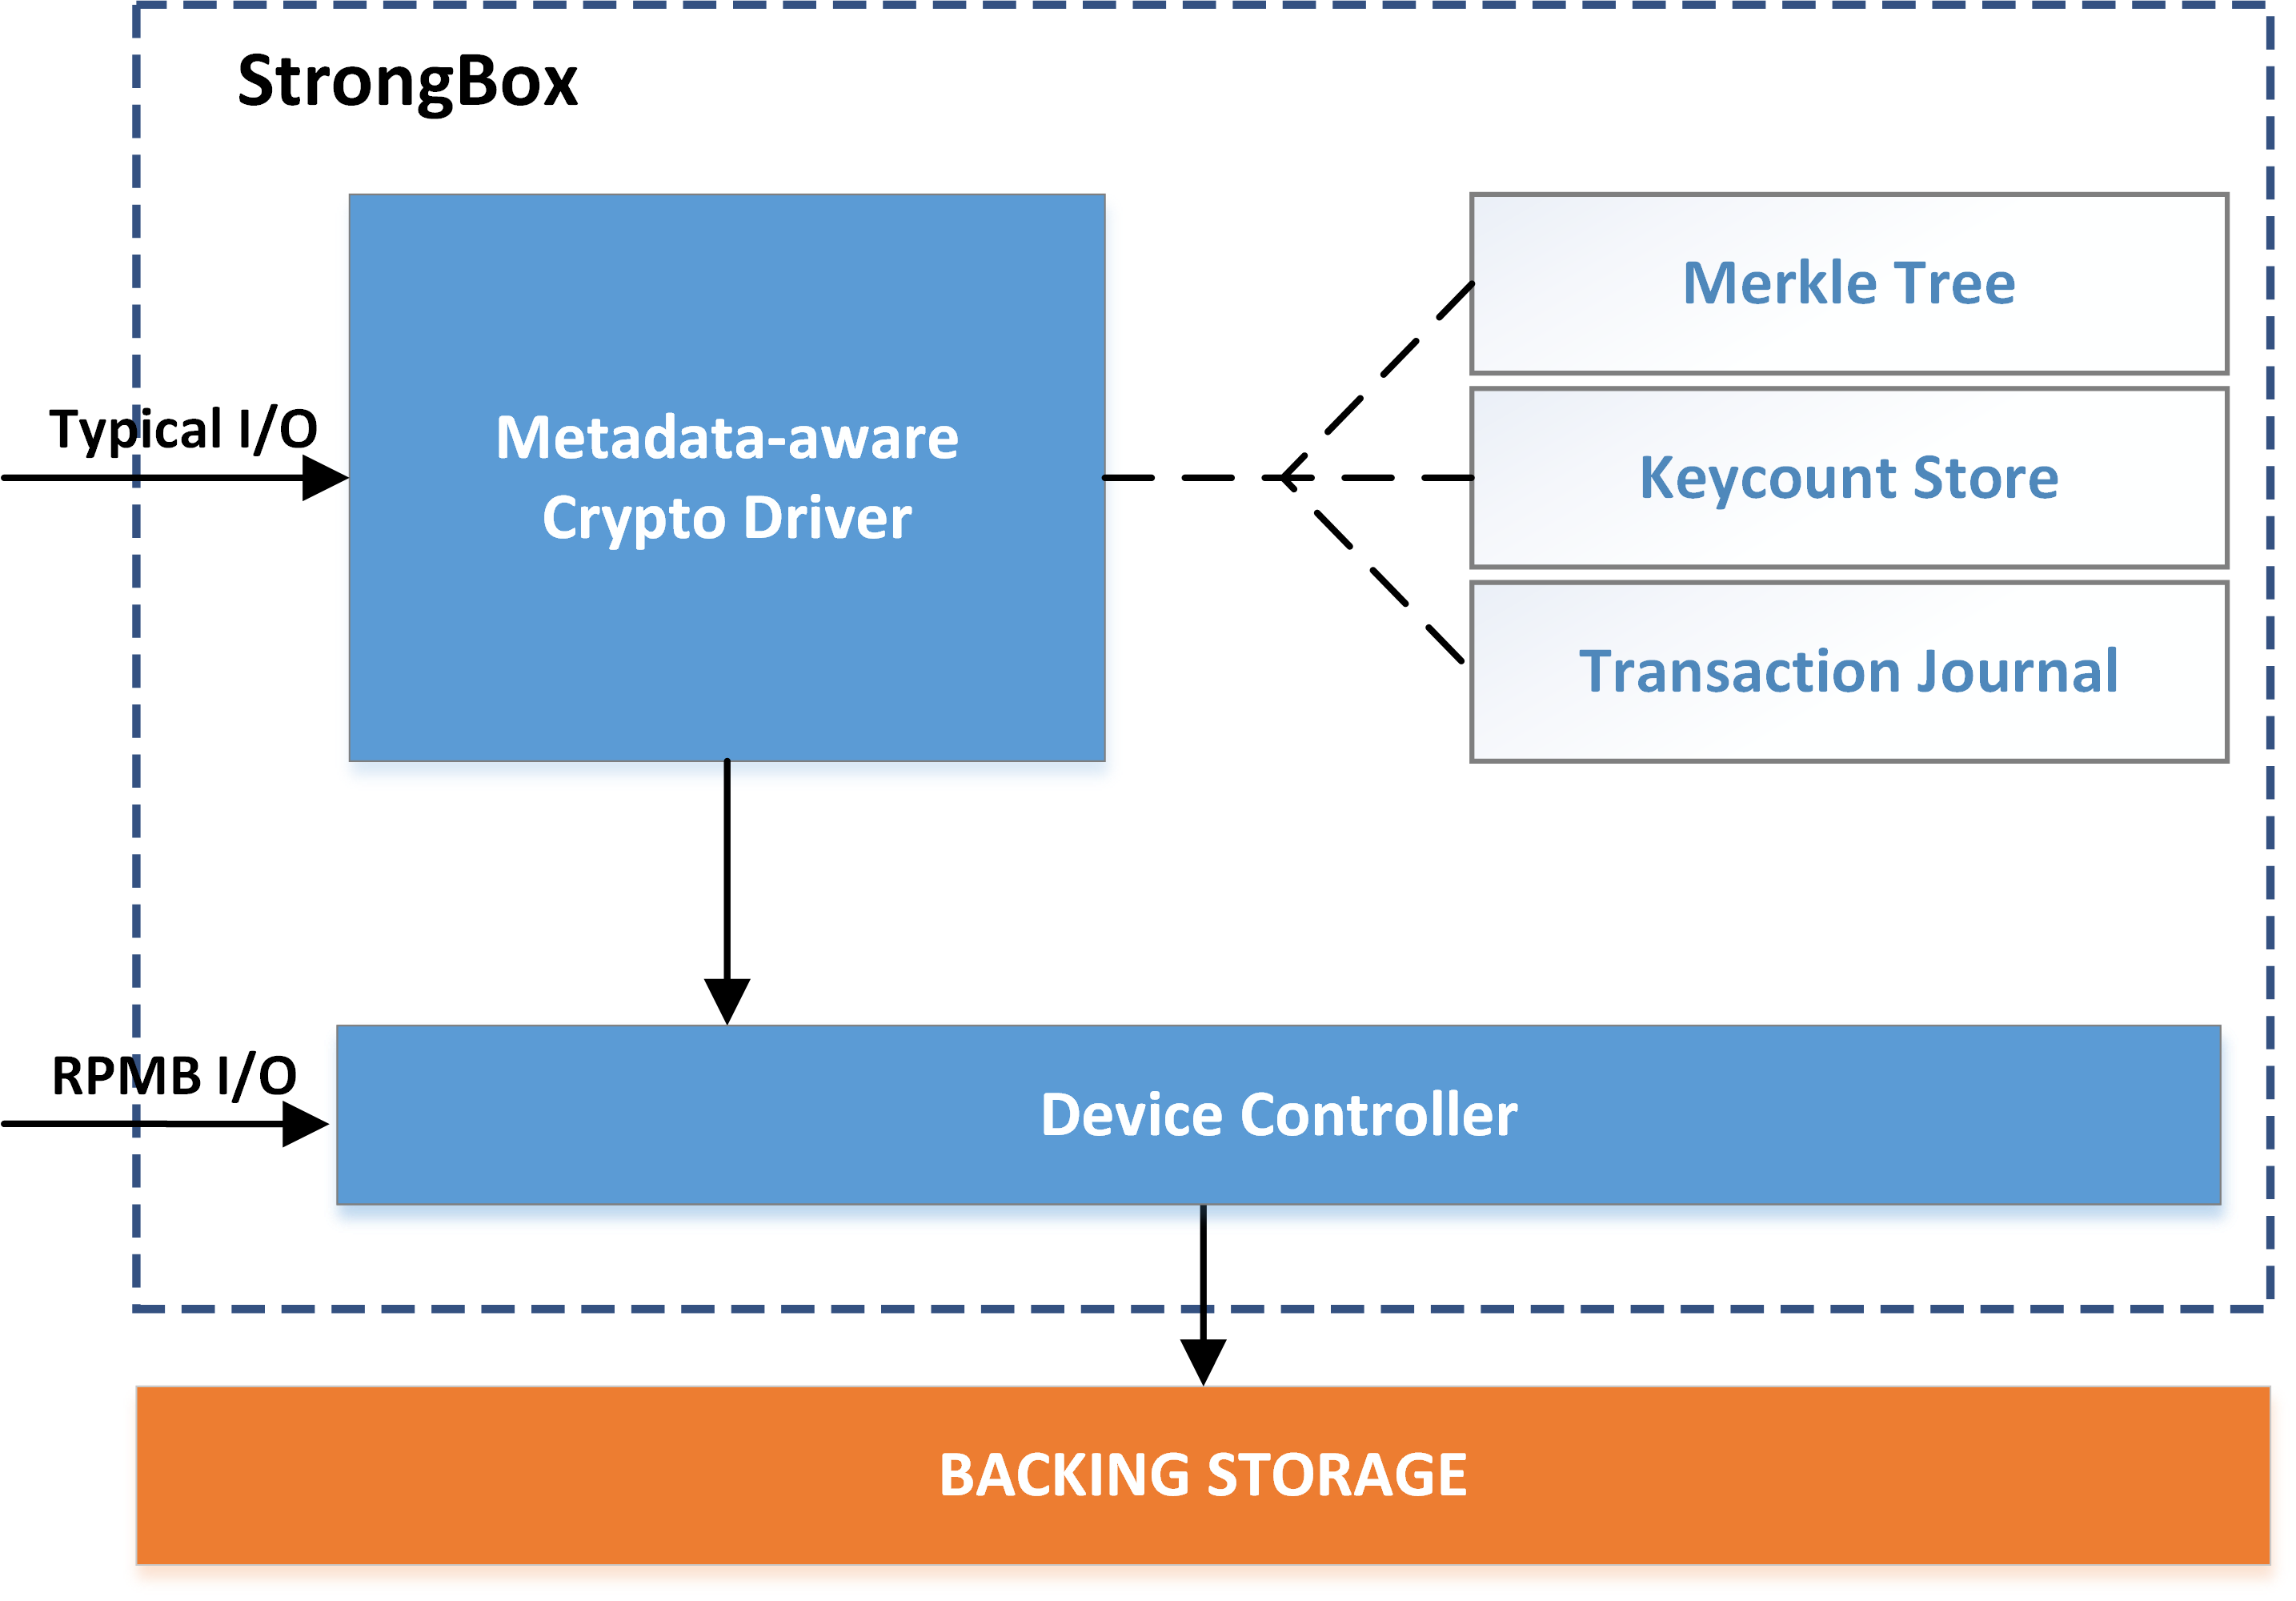
\includegraphics[width=0.8\linewidth]{overview.png}
   \caption{Overview of the StrongBox construction.}\label{fig:overview}
\end{figure}

\section{StrongBox System Design}\label{sec:design}

StrongBox acts as a translation layer sitting between the drive and the
operating system. It provides confidentiality and integrity guarantees while
minimizing performance loss due to metadata management overhead. StrongBox
accomplishes this by leveraging the speed of stream ciphers over the AES block
cipher and taking advantage of the append-mostly nature of Log-structured
Filesystems (LFS) and modern Flash Translation Layers (FTL)~\cite{SSD}.

Hence, there are several locations where StrongBox could be implemented in the
system stack. StrongBox could be integrated into an LFS kernel module
itself---\eg F2FS---specifically leveraging the flexibility of the Virtual
Filesystem Switch (VFS). StrongBox could be implemented as an actual block
device, or virtual block device layered atop a physical block device; the latter
is where we chose to implement our prototype. StrongBox could even be
implemented within the SSD drive controller's FTL, which handles scatter gather,
garbage collection, wear-leveling, etc.

\figref{overview} illustrates StrongBox's design. StrongBox's metadata is
encapsulated in four components: an in-memory \emph{Merkle Tree} and two
drive-backed byte arrays---the \emph{Keycount Store} and the \emph{Transaction
Journal}---and a persistent monotonic counter we implement with the \emph{Replay
Protected Memory Block} or RPMB. All four are integrated into the
\emph{Cryptographic Driver}, which handles data encryption, verification, and
decryption during interactions with the underlying backing store. These
interactions take place while fulfilling high-level I/O requests received from
the LFS. The \emph{Device Controller} handles low-level I/O between
StrongBox and the backing store.

The rest of this section describes the components referenced in
\figref{overview}. Specifically: we first describe the backing store and
StrongBox's layout for data and metadata. This is followed by an exploration of
the cryptographic driver and how it interacts with that metadata, the role of
the device controller, an overview of rekeying in the backing store, and further
considerations to ensure confidentiality in the case of rollbacks and related
attacks.

\subsection{Backing Store Function and Layout}

The backing store is the storage media on which StrongBox operates.
\figref{backstore} illustrates StrongBox's layout on this store.

\begin{figure}[t]
 \centering
  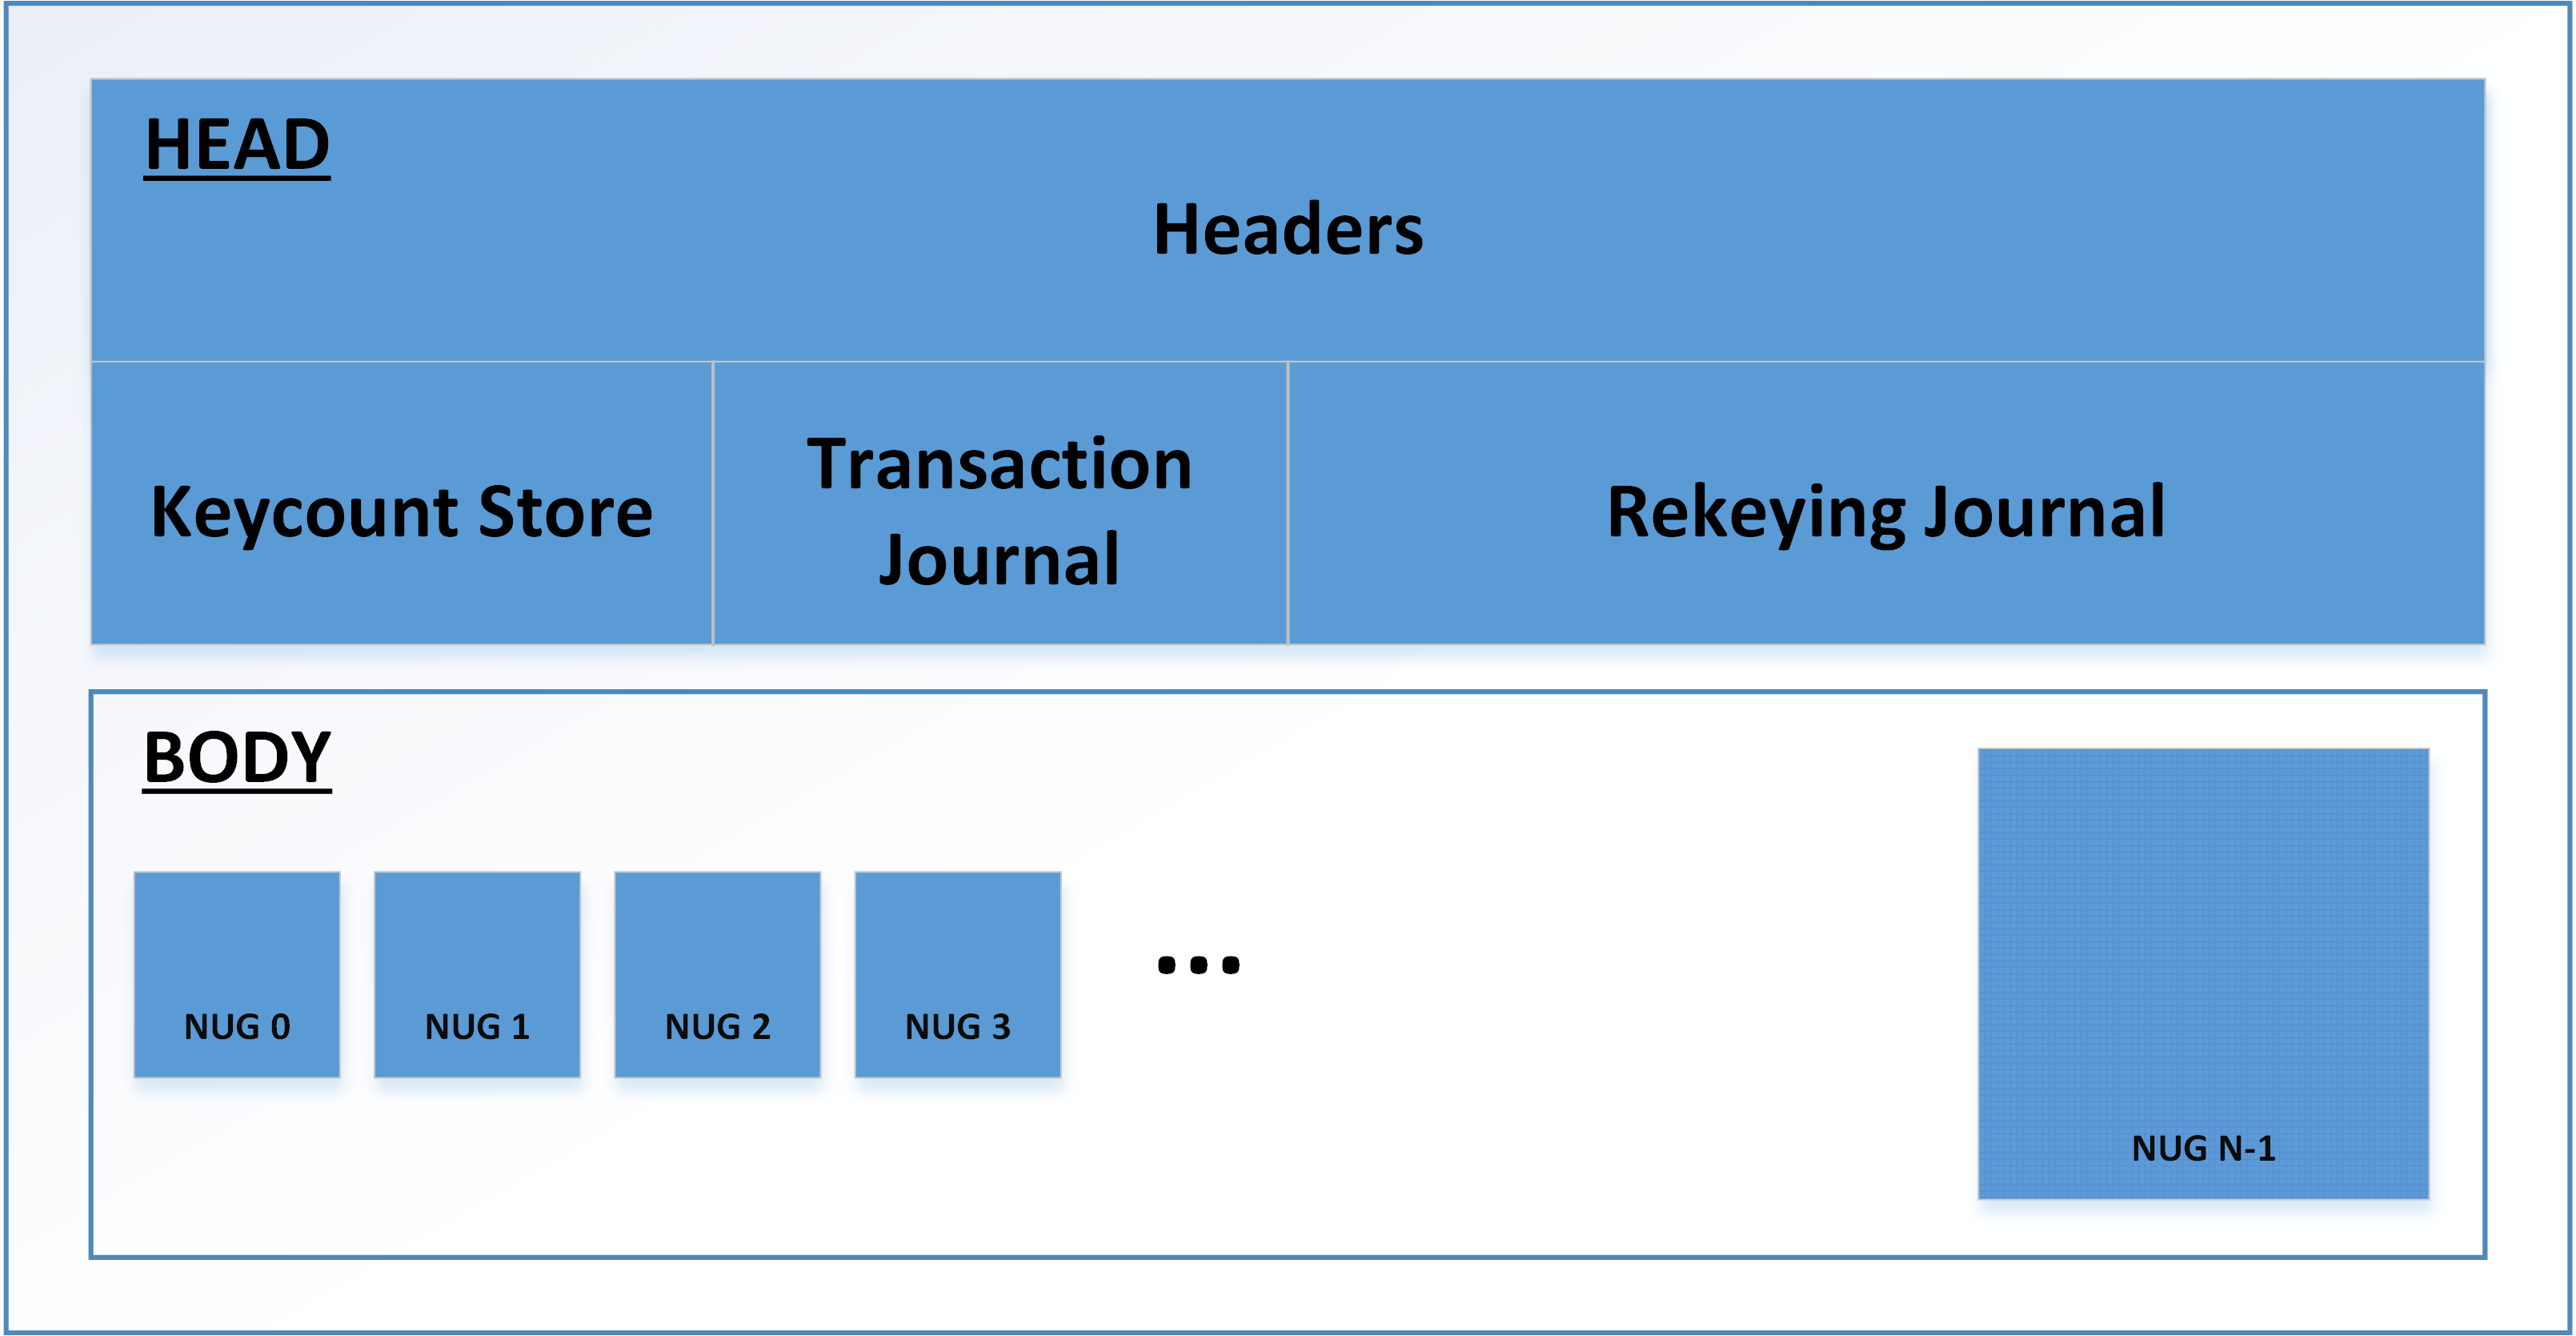
\includegraphics[width=0.8\linewidth]{backstore.png}
   \caption{Layout of StrongBox's backing storage.}\label{fig:backstore}
\end{figure}

In the \textit{body} section of the backing store layout, end-user data is
partitioned into a series of same-size \emph{logical blocks}. These are distinct
from the concept of \emph{physical drive blocks}, which are collections of one
or more drive sectors. To make this distinction clear, we refer to these wider
logical blocks as \emph{nuggets}, marked \textit{NUG} in the Body section of
\figref{backstore}. Hence, a nugget consists of one or more physical drive
blocks, depending on its configured size. Each nugget is subdivided into a
constant number of sub-blocks we refer to as \emph{flakes}.

The reason for these nugget/flake divisions are two-fold:

\begin{enumerate}

\item To track, detect, and handle overwrites and

\item To limit the maximum length of any plaintexts operated on by the
cryptographic driver, decreasing the overhead incurred per I/O operation and per
overwrite.

\end{enumerate}

% Describe how the components in fig 1 are represented on drive and how
% they play into the overall design WITHOUT naming them

Considering the first item, we are required to keep track of writes so that we
may detect when an overwrite occurs. Flakes are key to this tracking. When a
request comes in to write to one or more flakes in a nugget, StrongBox marks the
affected flakes as ``flagged''. Here, ``flagged'' implies that another write to
some portion of that flake would constitute an overwrite. If a new request comes
in to write to one or more of those same flakes another time, StrongBox triggers
a ``rekeying'' procedure over the entire nugget to safely overwrite the old data
in those flakes. This rekeying procedure is necessarily time consuming,
ballooning the overhead of overwrites translated by StrongBox.

Considering the second item, nugget size here governs the granularity of
rekeying while flake size governs granularity when identifying overwrites. A
larger nugget size will increase the penalty incurred with rekeying (you're
re-encrypting a larger number of bytes) while a smaller nugget size will increase
the quantity of nuggets needing to be rekeyed when an overwrite is detected as
well as increase the amount of metadata stored on drive and in memory. On the
other hand, a larger flake size will increase the number of times an incoming
write is seen as an overwrite, with a non-optimal nugget-sized flake requiring a
rekeying on \emph{every write}. A smaller flake size will increase the amount of
metadata stored on drive and in memory.

The size and structure of that metadata is described in greater detail
throughout the rest of this section.

The \textit{head} section of the backing store layout contains the metadata
written to drive during StrongBox's initialization. These headers govern
StrongBox's operation and are, in order:

\begin{enumerate}

\item VERSION, 4 bytes; specifies the StrongBox version originally used to
initialize the backing store

\item SALT, 16 bytes; the salt used in part to derive the global master secret

\item MTRH, 32 bytes; the hash of the Merkle Tree root

\item TPMGLOBALVER, 8 bytes; the monotonic global version count, parity in
hardware-supported secure storage

\item VERIFICATION, 32 bytes; used to determine if the key derived from a
password is correct

\item NUMNUGGETS, 4 bytes; the number of nuggets contained by the backing
store

\item FLAKESPERNUGGET, 4 bytes; the number of flakes/nugget

\item FLAKESIZE, 4 bytes; the size of each flake, in bytes

\item INITIALIZED, 1 byte; used to determine if the backing store has been
properly initialized

\item REKEYING, 4 bytes; the index of the nugget in need of rekeying if there
is a pending rekeying procedure

\end{enumerate}

After the headers, two byte arrays are stored in the Head section: one
of $N$ 8-byte integer \textit{keycounts} and one of $N$ $\ceil{P /
  8}$-byte \textit{transaction journal entries}, where $N$ is the
number of nuggets and $P$ is the number of flakes per nugget.

Finally, the \emph{Rekeying Journal} is stored at the end of the Head section.
The rekeying journal is where nuggets and their associated metadata are
transiently written, enabling StrongBox to resume rekeying in the event that it
is interrupted during the rekeying procedure.

\subsection{Metadata-aware Cryptographic Driver}

The cryptographic driver coordinates StrongBox's disparate components.
Its primary function is to map incoming reads and writes to their
proper destinations in the backing store, applying our chosen stream
cipher and message authentication code to encrypt, verify, and decrypt
data on the fly with consideration for metadata management.

When a read request is received, it is first partitioned into affected
nuggets; \eg a read that spans two nuggets is partitioned in half.
For each nugget affected, we calculate which flakes are touched by the
request. We then verify the contents of those flakes. If all the
flakes are valid, whatever subset of data that was requested by the
user is decrypted and returned. \algoref{read} details StrongBox's
read operation.

Like reads, when a write request is received, the request is first
partitioned with respect to affected nuggets. For each affected
nugget, we calculate which flakes are touched by the request and then
check if any of those flakes are marked as flagged in the transaction
journal. If one or more of them have been marked flagged, we trigger
rekeying for this specific nugget (see: \algoref{rekeying}) and end
there. Otherwise, we mark these touched flakes as flagged in the
transaction journal. We then iterate over these touched flakes. For
the first and last flakes touched by the write request, we execute an
internal read request (see: \algoref{read}) to both obtain the flake
data and verify that data with the Merkle Tree. We then overwrite
every touched flake with the data from the requested operation, update
the Merkle Tree to reflect this change, encrypt and write out the new
flake data, and commit all corresponding metadata. \algoref{write}
details StrongBox's write operation.

\begin{algorithm}[t]
%\floatname{algorithm}{Algorithm}
\caption{StrongBox handling an incoming read request.}\label{algo:read}
{\footnotesize 
\begin{algorithmic}[1]
\Require The read request is over a contiguous segment of the backing
store
\Require $\ell, \ell' \leftarrow$ read requested length
\Require $\aleph \leftarrow$ master secret
\Require $n_{index} \leftarrow$ first nugget index to be read
\State $data \leftarrow$ \emph{empty}
\While{$\ell \neq 0$}
    \State $k_{n_{index}} \leftarrow GenKey_{nugget}(n_{index}, \aleph)$
    \State Fetch nugget keycount $n_{kc}$ from Keycount Store.
    \State Calculate indices touched by request: $f_{first}$, $f_{last}$
    \State $n_{flakedat} \leftarrow ReadFlakes(f_{first},\dots,f_{last})$
    \For{$f_{current} = f_{first}$ \textbf{to} $f_{last}$}
        \State $k_{f_{current}} \leftarrow GenKey_{flake}(k_{n_{index}},
        f_{current}, n_{kc})$
        \State $tag_{f_{current}} \leftarrow GenMac(k_{f_{current}},
        n_{flakedat}[f_{current}])$
        \State Verify $tag_{f_{current}}$ in Merkle Tree.
    \EndFor 
    \LineComment{(\textbf{*}) denotes requested subset of nugget data}
    \State $data \leftarrow data + Decrypt(*n_{flakedat}, k_{n_{index}},
    n_{kc})$
    \State $\ell \leftarrow \ell - \|*n_{flakedat}\|$
    \State $n_{index} \leftarrow n_{index} + 1$
\EndWhile 
\\\Return $data$ \Comment{Fulfill the read request}
\Ensure $\|data\| <= \ell'$ 
\Ensure $\ell = 0$
\vskip -1.5em
\end{algorithmic}
}
\end{algorithm}

\begin{algorithm}[t]
%\floatname{algorithm}
\caption{StrongBox handling an incoming write request.}\label{algo:write}
{\footnotesize 
\begin{algorithmic}[1]
\Require The write request is to a contiguous segment of the backing store
\Require $\ell, \ell' \leftarrow$ write requested length
\Require $\aleph \leftarrow$ master secret
\Require $data \leftarrow$ cleartext data to be written
\Require $n_{index} \leftarrow$ first nugget index to be affected
\State Increment secure counter: by 2 if we recovered from a crash, else 1
\While{$\ell \neq 0$}
    \State Calculate indices touched by request: $f_{first}$, $f_{last}$
    \If{Transaction Journal entries for $f_{first},\dots,f_{last} \neq 0$}
        \State Trigger rekeying procedure (see: \algoref{rekeying}).
        \State \textbf{continue}
    \EndIf 
    \State Set Transaction Journal entries for $f_{first},\dots,f_{last}$ to 1
    \State $k_{n_{index}} \leftarrow GenKey_{nugget}(n_{index}, \aleph)$
    \State Fetch nugget keycount $n_{kc}$ from Keycount Store.
    \For{$f_{current} = f_{first}$ \textbf{to} $f_{last}$}
        \State $n_{flakedat} \leftarrow $ \textit{empty}
        \If{$f_{current} == f_{first} \| f_{current} == f_{last}$}
            \State $n_{flakedat} \leftarrow CryptedRead(\textit{FSIZE}, \aleph,
            n_{index}$@$f_{offset})$
        \EndIf 
        \State $n_{flakedat} \leftarrow Encrypt(n_{flakedat}, k_{n_{index}},
        n_{kc})$
        \State $k_{f_{current}} \leftarrow GenKey_{flake}(k_{n_{index}},
        f_{current}, n_{kc})$
        \State $tag_{f_{current}} \leftarrow GenMac(k_{f_{current}},
        n_{flakedat})$
        \State Update new $tag_{f_{current}}$ in Merkle Tree.
        \State $WriteFlake(f_{current}, n_{flakedat})$
        \\\LineComment{(\textbf{*}) denotes requested subset of nugget data if
        applicable}
        \State $\ell \leftarrow \ell - \|*n_{flakedat}\|$
    \EndFor 
    \State $n_{index} \leftarrow n_{index} + 1$
\EndWhile 
\State Update and commit metadata and headers
\Ensure $\ell = 0$
\vskip -1.5em
\end{algorithmic}
}
\end{algorithm}

% Algorithmic analysis?

\subsubsection{Transaction Journal}

An overwrite breaks the security guarantee offered by any stream
cipher. To prevent this failure, StrongBox tracks incoming write
requests to prevent overwrites. This tracking is done with the
transaction journal, featured in \figref{overview}.

% Describe how this component meets that need
The transaction journal consists of $N$ $\ceil{P / 8}$-byte bit
vectors where $N$ is the number of nuggets and $P$ is the number of
flakes per nugget. A bit vector $v$ contains at least $P$ bits $v = \{
b_0, b_1, b_2, \dots, b_{P-1}, \dots \}$, with extra bits ignored.
Each vector is associated with a nugget and each bit with a flake
belonging to that nugget. When an incoming write request occurs, the
corresponding bit vector is updated (set to 1) to reflect the new
flagged state of those flakes.

% Describe briefly TJ's relation to writes: when it's referenced and when it's
% changed
The transaction journal is referenced during each write request, where
it is updated to reflect the state of the nugget and checked to ensure
the operation does not constitute an overwrite. If the operation
\textit{does} constitute an overwrite, StrongBox triggers a rekeying
procedure for the entire nugget before safely completing the request.

\subsubsection{Merkle Tree}\label{sec:merkle}

Tracking writes with the transaction journal may stymie a passive
attacker by preventing explicit overwrites, but a sufficiently
motivated active attacker could resort to all manner of cut-and-paste
tactics with nuggets, flakes, and even blocks and sectors. If, for
example, an attacker purposefully zeroed-out the transaction journal
entry pertaining to a specific nugget in some out-of-band
manner---such as when StrongBox is shut down and then later
re-initialized with the same backing store---StrongBox would consider
any successive incoming writes as if the nugget were in a completely
clean state, even though it actually is not. This attack would force
StrongBox to make compromising overwrites. To prevent such attacks, we
must ensure that the backing store is always in a valid state. More
concretely: we must provide an integrity guarantee on top of a
confidentiality guarantee.

StrongBox uses our chosen Message Authentication Code (MAC) generating algorithm
and each flake's unique key to generate a per-flake MAC tag (``MACed''). The
purpose of this tag is to authenticate flake data and confirm that it has not
been tampered with. Each tag is then appended to the Merkle Tree along with
StrongBox's metadata.

The transaction journal entries are handled specially in that the bit
vectors are MACed and the result is appended to the Merkle Tree. This is done to
save space.

The Merkle Tree then ties the integrity of any single flake to the integrity of
the system as a whole such that if the former fails, \ie{there is a MAC tag
mismatch for any particular flake}, the latter immediately and obviously fails.

\subsubsection{Keycount Store}

To prevent a many-time pad attack, each nugget is assigned its own
form of nonce we refer to as a \emph{keycount}. The keycount store in
\figref{overview} represents a byte-array containing $N$ 8-byte
integer keycounts indexed to each nugget. Along with acting as the
per-nugget nonce consumed by the stream cipher, the keycount is used
to derive the per-flake unique subkeys used in MAC tag generation.

\subsubsection{Rekeying Procedure}

When a write request would constitute an overwrite, StrongBox will
trigger a rekeying process instead of executing the write normally.
This rekeying process allows the write to proceed without causing a
catastrophic confidentiality violation.

When rekeying begins, the nugget in question is loaded into memory and
decrypted. The target data is written into its proper offset in this decrypted
nugget. The nugget is then encrypted, this time with a different nonce
(\textit{keycount + 1}), and written to the backing store, replacing the
outdated nugget data. See: \algoref{rekeying}.

\begin{algorithm}[t]
%\floatname{algorithm}
\caption{StrongBox rekeying process.}\label{algo:rekeying}
{\footnotesize 
\begin{algorithmic}[1]
\Require The original write applied to a contiguous backing store segment
\Require $\ell \leftarrow$ write requested length
\Require $\aleph \leftarrow$ master secret
\Require $data \leftarrow$ cleartext data to be written
\Require $n_{index} \leftarrow$ nugget rekeying target

\Comment{Read in and decrypt the entire nugget}
\State $n_{nuggetdat} \leftarrow CryptedRead(\textit{NSIZE}, \aleph, n_{index})$
\State Calculate indices touched by request: $f_{first}$, $f_{last}$
\State Write $data$ into $n_{nuggetdat}$ at proper offset with length $\ell$
\State Set Transaction Journal entries for $f_{first},\dots,f_{last}$ to 1
\State $k_{n_{index}} \leftarrow GenKey_{nugget}(n_{index}, \aleph)$
\State Fetch nugget keycount $n_{kc}$ from Keycount Store. Increment it by one.
\State $n_{nuggetdat} \leftarrow Encrypt(n_{nuggetdat}, k_{n_{index}}, n_{kc})$
\State Commit $n_{nuggetdat}$ to the backing store

\Comment{Iterate over all flakes in the nugget}
\ForAll{flakes $f_{current}$ \textbf{in} $n_{index}$}
    \State $k_{f_{current}} \leftarrow GenKey_{flake}(k_{n_{index}},
    f_{current}, n_{kc})$
    \State Copy $f_{current}$ data from $n_{nuggetdat} \rightarrow n_{flakedat}$
    \State $tag_{f_{current}} \leftarrow GenMac(k_{f_{current}}, n_{flakedat})$
    \State Update new $tag_{f_{current}}$ in Merkle Tree.
\EndFor 
\State Update and commit metadata and headers
\vskip -1.5em
\end{algorithmic}
}
\end{algorithm}

\subsection{Defending Against Rollback Attacks}

To prevent StrongBox from making overwrites, the status of each flake
is tracked and overwrites trigger a rekeying procedure. Tracking flake
status alone is not enough, however. An attacker could take a snapshot
of the backing store in its current state and then easily rollback to
a previously valid state. At this point, the attacker could have
StrongBox make writes that it does not recognize as overwrites.

With AES-XTS, the threat posed by rolling the backing store to a
previously valid state is outside of its threat model. Despite this,
data confidentiality guaranteed by AES-XTS holds in the event of a
rollback, even if integrity is violated.

StrongBox uses a monotonic global version counter to detect rollbacks.
When a rollback is detected, StrongBox will refuse to initialize
unless forced, using root permission. Whenever a write request is
completed, this global version counter is committed to the backing
store, committed to secure hardware, and updated in the in-memory
Merkle Tree.

\subsection{Recovering from Inconsistent State}

If StrongBox is interrupted during operation, the backing store---consisting of
user data and StrongBox metadata---will be left in an inconsistent state.
StrongBox relies on the overlying filesystem \eg{F2FS} to manage user-data
recovery, which is what these filesystems are designed to do and do well. We
detail how StrongBox handles its own inconsistent metadata.

Let $c$ be the value of the on-chip monotonic global version counter and $d$ be
the value of the on-drive global version counter header (TPMGLOBALVER). Consider
the following:

\begin{itemize}

\item \emph{$c == d$ and MTRH is consistent:} StrongBox is operating
  normally and will mount without issue.

\item \emph{$c<d$ or $c == d$ but MTRH is inconsistent:} Since the
  global version counter is updated before any write, this case cannot
  be reached unless the backing store was manipulated by an attacker.
  So, StrongBox will refuse to initialize and cannot be force mounted.

\item \emph{$c > d + 1$:} Since the global version counter is updated
  once per write, this case cannot be reached unless the backing store
  was rolled back or otherwise manipulated by an attacker. In this
  case, the root user is warned and StrongBox will refuse to
  initialize and cannot be force mounted unless the MTRH is
  consistent. We allow the root user to force mount here if the root
  user initiated the rollback themselves, such as when recovering from
  a drive backup.

\item \emph{$c == d + 1$:} In this case, StrongBox likely crashed
  during a write, perhaps during an attempted rekeying. If the
  rekeying journal is empty or the system cannot complete the rekeying
  and/or bring the MTRH into a consistent state, the root user is
  warned and allowed to force mount. Otherwise, StrongBox will not
  initialize.

\end{itemize}

For subsequent rekeying efforts in the latter two cases, rather than
incrementing the corresponding keystore counters by 1 during rekeying,
they will be incremented by 2. This is done to prevent potential reuse
of any derived nugget keys that might have been in use right before
StrongBox crashed.

When StrongBox can detect tampering, it will not initialize. When StrongBox
cannot distinguish between tampering and crash, it offers the root user a choice
to force mount. Thus, an attacker could force a crash and use root access to
force mount. We assume, however, that if an attacker has root access to a
device, its security is already compromised.

\section{StrongBox Implementation}\label{sec:implementation}

Our implementation of StrongBox is comprised of 5000 lines of C code. StrongBox
uses OpenSSL version 1.0.2 and LibSodium version 1.0.12 for its ChaCha20,
Argon2, Blake2, and AES-XTS implementations, likewise implemented in C. The
SHA-256 Merkle Tree implementation is borrowed from the Secure Block Device
library~\cite{SBD}. StrongBox's implementation is available as
open-source.\footnote{\StrongBoxURI}

To reduce the complexity of the experimental setup, establish a fair baseline,
and allow StrongBox to run in user space, we use a BUSE~\cite{BUSE} virtual
block device. BUSE is a thin (200 LOC) wrapper around the standard Linux Network
Block Device (NBD), which allows a machine to serve requests for reads and
writes to virtual block devices exposed via domain socket. We built StrongBox on
top of BUSE/NBD because a simple block device in user space allows for quick
experimentation and rapid prototyping. It is not required for a proper
implementation.

\subsection{Deriving Subkeys}
The cryptographic driver requires a shared master secret. The
derivation of this master secret is implementation specific and has no
impact on performance as it is completed during StrongBox's
initialization. Our implementation uses the Argon2 KDF to derive a
master secret from a given password with an acceptable time-memory
trade-off.

% Describe deriving the nugget keys from the master secret
To assign each nugget its own unique keystream, that nugget requires a
unique key and associated nonce. We derive these nugget subkeys from
the master secret during StrongBox's initialization. To guarantee the
backing store's integrity, each flake is tagged with a MAC. We use
Poly1305, accepting a 32-byte one-time key and a plaintext of
arbitrary length to generate tags. These one-time flake subkeys are
derived from their respective nugget subkeys.

\subsection{A Secure, Persistent, Monotonic Counter} 
Our target platform uses an embedded Multi-Media Card (eMMC) as a
backing store. In addition to boot and user data partitions, the eMMC
standard includes a secure storage partition called a Replay Protected
Memory Block (RPMB)~\cite{eMMC-standard}. The RPMB partition's size
is configurable to be at most 16MB (32MB on some Samsung
devices)~\cite{RPMB}. All read and write commands issued to the RPMB
must be authenticated by a key burned into write-once storage
(typically eFUSE) during some one-time, secure initialization process.

To implement rollback protection on top of the RPMB, the key for
authenticating RPMB commands can be contained in TEE sealed storage or
derived from the TPM. For this implementation, StrongBox requires
interaction with TPM/TEE secure storage only at mount time, where the
authentication key can be retrieved and cached for the duration of
StrongBox's lifetime. With the cached key on hand, our implementation
makes traditional IOCTL calls to read and write global version counter
data to the RPMB eMMC partition, enforcing the invariant that it only
increase monotonically.

Our design is not dependent on the eMMC standard, however. Trusted
hardware mechanisms other than the eMMC RPMB partition, including
TPMs, support secure, persistent storage and/or monotonic counters
directly. These can be adapted for use with StrongBox just as well.

There are two practical concerns we must address while implementing
the secure counter: wear and performance overhead. Wear is a concern
because the counter is implemented in non-volatile storage. The RPMB
implements all the same wear protection mechanisms that are used to
store user-data~\cite{eMMC-standard}. Additionally, StrongBox writes
to the global version counter once per write to user-data. Given that
the eMMC implements the same wear protection for the RPMB and user
data, and that the ratio of writes to these areas is 1:1, we expect
StrongBox places no additional wear burden on the hardware. Further,
with the JEDEC spec suggesting RPMB implementations use more durable
and faster single-level NAND flash cells rather than cheaper and
slower multi-level NAND flash cells \cite{eMMC-standard,RPMB}, the
RPMB partition will likely outlive and outperform the user-data
portion of the eMMC.

In terms of performance overhead, updating the global version counter
requires making one 64-bit authenticated write per user-data write. As
user-data writes are almost always substantially larger, we see no
significant overhead from the using the RPMB to store the secure
counter.

\subsection{LFS Garbage Collection}

An LFS attempts to write to a drive sequentially in an append-only fashion, as
if writing to a log. This requires large amounts of contiguous space, called
\emph{segments}. Since any backing store is necessarily finite, an LFS can only
append so much data before it runs out of space. When this occurs, the LFS
triggers a \emph{segment cleaning algorithm} to erase outdated data and
compress the remainder of the log into as few segments as
possible~\cite{LFS,F2FS}. This procedure is known more broadly as \emph{garbage
collection}~\cite{F2FS}.

In the context of StrongBox, garbage collection could potentially incur high
overhead. The procedure itself would, with its every write, require a rekeying
of any affected nuggets. Worse, every proceeding write would appear to StrongBox
as if it were an overwrite, since there is no way for StrongBox to know that the
LFS triggered garbage collection internally.

In practice, modern production LFSes are optimized to perform garbage collection
as few times as possible~\cite{F2FS}. Further, they often perform garbage
collection in a background thread that triggers when the filesystem is idle and
only perform expensive on-demand garbage collection when the backing store is
nearing capacity~\cite{F2FS, NILFS}. We leave garbage collection turned on for
all of our tests and see no substantial performance degradation from this
process because it is scheduled not to interfere with user I/O.

\subsection{Overhead}

StrongBox stores metadata on the drive it is encrypting (see
\figref{backstore}). This metadata should be small compared to the user data.
Our implementation uses 4KB flakes, 256 flakes/nugget, and 1024 nuggets per GB
of user data. Given the flake and nugget overhead, this configuration requires
just over 40KB of metadata per 1 GB of user data. There is an additional, single
static header that requires just over 200 bytes. \emph{Thus StrongBox's overhead
in terms of storage is less than one hundredth of a percent.}

\section{Evaluation}\label{sec:evaluation}

\subsection{Experimental Setup}

We implement a prototype of StrongBox on a Hardkernel Odroid XU3 ARM big.LITTLE
system (Samsung Exynos5422 A15 and A7 quad core CPUs, 2Gbyte LPDDR3 RAM at 933
MHz, eMMC5.0 HS400 backing store) running Ubuntu Trusty 14.04 LTS, kernel
version 3.10.58. The maximum theoretical memory bandwidth for this model is
14.9GB/s\@. Observed maximum memory bandwidth is 4.5GB/s.

\subsection{Experimental Methodology}

In this section we seek to answer three questions:
\begin{enumerate}
\item What is StrongBox's overhead when compared to dm-crypt AES-XTS?
\item How does StrongBox under an LFS (\ie F2FS) configuration compare to
the popular dm-crypt under Ext4 configuration?
\item Where does StrongBox derive its performance gains? Implementation? Choice
of cipher?
%\item How does StrongBox perform when the backing store is nearly full?
\end{enumerate}

To evaluate StrongBox's performance, we measure the latency
(seconds/milliseconds per operation) of both sequential and random
read and write I/O operations across four different standard Linux
filesystems: NILFS2, F2FS, Ext4 in ordered journaling mode, and Ext4
in full journaling mode. The I/O operations are performed using file
sizes between 4KB and 40MB. These files were populated with random
data. The experiments are performed using a 1GB standard Linux ramdisk
(tmpfs) as the ultimate backing store.

For sequential F2FS specifically, we include latency measurements dealing
with a file size $2.5\times$ the size of available DRAM, \ie
5GB, supported by a distinct tmpfs backing store swapped into memory.

Ext4's default is ordered journaling mode (\texttt{data=ordered}),
where metadata is committed to the filesystem's journal while the
actual data is written through to the main filesystem. Given a crash,
the filesystem uses the journal to avoid damage and recover to a
consistent state. Full journaling mode (\texttt{data=journal})
journals both metadata and the filesystem's actual data---essentially
a double write-back for each write operation. Given a crash, the
journal can replay entire I/O events so that both the filesystem and
its data can be recovered. We include both modes of Ext4 to further
explore the impact of frequent overwrites against StrongBox.

The experiment consists of reading and writing each file in its
entirety 30 times sequentially, and then reading and writing random
portions of each file 30 times. In both cases, the same amount of data
is read and written per file. The median latency is taken per result
set. We chose 30 read/write operations (10 read/write operations
repeated three times each) to handle potential variation. The Linux
page cache is dropped before every read operation, each file is
opened in synchronous I/O mode via \texttt{O\_SYNC}, and we rely on
non-buffered \texttt{read()}/\texttt{write()} system calls. A
high-level I/O size of 128KB was used for all read and write calls
that hit the filesystems; however, the I/O requests being made at the
block device layer varied between 4KB and 128KB depending on the
filesystem under test.

The experiment is repeated on each filesystem in three different
configurations:
\begin{enumerate}
\item \textit{unencrypted}: Filesystem mounted atop a BUSE virtual block
  device set up to immediately pass through any incoming I/O requests straight
  to the backing store. We use this as the baseline measurement of the
  filesystem's performance without any encryption.
\item \textit{StrongBox}: Filesystem mounted atop a BUSE virtual block
  device provided by our StrongBox implementation to perform full-drive
  encryption.
\item \textit{dm-crypt}: Filesystem mounted atop a Device Mapper
 ~\cite{LinuxDeviceMapper} higher-level virtual block device provided by
  dm-crypt to perform full-drive encryption, which itself is mounted atop a
  BUSE virtual block device with pass through behavior identical to the device
  used in the baseline configuration. dm-crypt was configured to use AES-XTS as
  its full-drive encryption algorithm. All other parameters were left at their
  default values.
\end{enumerate}

\figref{microbench-f2fs} compares StrongBox to dm-crypt under the F2FS
filesystem. The gamut of result sets over different filesystems can
be seen in \figref{microbench-gamut}. \figref{microbench-ext4}
compares Ext4 with dm-crypt to F2FS with StrongBox.

\begin{figure}[ht]
    \textbf{StrongBox vs dm-crypt AES-XTS: F2FS Test}\par\medskip
    \begin{subfigure}{\linewidth}
        \centering
        {\input{img/microbench-f2fs-sequential.tex}}
        \caption{Sequential I/O expanded F2FS result set.}\label{fig:microbench-f2fs-sequential}
    \end{subfigure}\\[1ex]
    \begin{subfigure}{\linewidth}
        \centering
        {\input{img/microbench-f2fs-random.tex}}
        \caption{Random I/O expanded F2FS result set.}\label{fig:microbench-f2fs-random}
    \end{subfigure}
    \caption{Test of the F2FS LFS mounted atop both dm-crypt and
      StrongBox; median latency of different sized whole file read and
      write operations normalized to unencrypted access. By harmonic
      mean, StrongBox is $1.72\times$ faster than dm-crypt for sequential reads
      and $1.27\times$ faster for sequential writes.}\label{fig:microbench-f2fs}
\end{figure}

\subsection{StrongBox Read Performance}

\figref{microbench-f2fs} shows the performance of StrongBox in comparison to
dm-crypt, both mounted with the F2FS filesystem. We see StrongBox improves on
the performance of dm-crypt's AES-XTS implementation across sequential and
random read operations on all file sizes. Specifically, $2.36\times$
(53.05m/22.48m) for sequential 5GB, $2.07\times$ (2.09s/1.00s) for sequential
40MB, $2.08\times$ (267.34ms/128.22ms) for sequential 5MB, $1.85\times$
(28.30ms/15.33ms) for sequential 512KB, and $1.03\times$ (0.95ms/0.86ms) for
sequential 4KB\@.

\figref{microbench-gamut} provides an expanded performance profile for
StrongBox, testing a gamut of filesystems broken down by workload file size. For
sequential reads across all filesystems and file sizes, StrongBox outperforms
dm-crypt. This is true even on the non-LFS Ext4 filesystems. Specifically, we
see read performance improvements over dm-crypt AES-XTS for 40MB sequential
reads of $2.02\times$ (2.15s/1.06s) for NILFS, $2.07\times$ (2.09s/1.00s) for
F2FS, $2.09\times$ (2.11s/1.01s) for Ext4 in ordered journaling mode, and
$2.06\times$ (2.11s/1.02s) for Ext4 in full journaling mode. For smaller file
sizes, the performance improvement is less pronounced. For 4KB reads we see
$1.28\times$ (1.62ms/1.26ms) for NILFS, $1.03\times$ (0.88ms/0.86ms) for F2FS,
$1.04\times$ (0.95ms/0.92ms) for Ext4 in ordered journaling mode, and
$1.07\times$ (0.97ms/0.91ms) for Ext4 in full journaling mode. When it comes to
random reads, we see virtually identical results save for 4KB reads, where
dm-crypt proved slightly more performant under the NILFS LFS at $1.12\times$
(1.73ms/1.54ms). This behavior is not observed with the more modern F2FS\@.

% \begin{figure*}[t]
%     \textbf{StrongBox Four Filesystems Test}\par\medskip
%     \centering
%     \begin{subfigure}{0.5\linewidth}
%         \centering
%         {\begin{tikzpicture}[baseline]

% XXX: update 0
\pgfmathsetmacro{\ymax}{2} % set the maximum y value
\pgfmathsetmacro{\ymaxbreak}{2.05} % set the y value at which overflow is drawn

\begin{groupplot}[
    group style={
        group name=plots,
        group size=1 by 1,
        xlabels at=edge top,
        xticklabels at=edge top,
        vertical sep=5pt,
    },
    axis x line*=top,
    xlabel near ticks,
    major x tick style=transparent,
    height=6cm,
    width=\linewidth,
    xmin=0, xmax=5,
    % enlarge y limits={value=0.2,upper},
    tick align=outside,
    tick style={white},
    ytick=\empty,
    xtick=\empty,
    xticklabels={},
    yticklabels={},
    % restrict y to domain*=0:2,
    clip=false,
]
\nextgroupplot[
    ylabel={\footnotesize Latency (normalized to dm-crypt)}, % XXX: update 1
    ylabel shift={6mm},
    ymin=0, ymax=1,
]
\end{groupplot}

\begin{groupplot}[
    group style={
        group name=plots,
        group size=1 by 1,
        xlabels at=edge bottom,
        xticklabels at=edge bottom,
        vertical sep=5pt
    },
    axis x line*=bottom,
    xlabel near ticks,
    major x tick style=transparent,
    height=6cm,
    width=\linewidth,
    %xmin=0, %xmax=2,
    xlabel={\footnotesize File Size (bytes)},
    symbolic x coords={4K,512K,5M,40M},
    xticklabels={\footnotesize{4K}, \footnotesize{512K}, \footnotesize{5M}, \footnotesize{40M}},
    xtick=data,
    enlarge x limits=0.2, % add some breathing room along the x axis's sides
    extra y ticks={1},
    extra y tick style={grid=major, grid style={dashed, black}},
    extra y tick label={ 1 },
    tick align=outside,
    tick style={ black },
    legend cell align=center,
    legend style={ column sep=1ex },
    ymajorgrids=true,
    grid style={ dotted, gray },
    every node near coord/.append style={font=\tiny},
    % magic to make the numbers appear above the overly long bars:
    visualization depends on={rawy \as \rawy}, % save original y values
    restrict y to domain*={ % now clip/restrict any y value to ymax
        \pgfkeysvalueof{/pgfplots/ymin}:\ymaxbreak
    },
    after end axis/.code={ % draw squiggly line indicating break
        \draw [semithick, white, decoration={snake,amplitude=0.1mm,segment length=0.75mm,post length=0.375mm}, decorate] (rel axis cs:0,1.01) -- (rel axis cs:1,1.01);
    },
    nodes near coords={\color{.!75!black}\pgfmathprintnumber\rawy}, % print the original y values (darkened in case they're too light)...
    nodes near coords greater equal only=\ymax, % ... but ONLY if they're >= ymax
    clip=false, % allow clip to protrude beyond ymax
    %
    % Custom stuff to edit per template
    % XXX: update 2
    ymin=0, ymax=\ymax,
    ytick={ 0, 0.5, 1.5, 2 },
    yticklabels={ 0, 0.5, 1.5, 2 },
]
\nextgroupplot[
    % XXX: update 3
    ybar=1pt, % change space between bars
    bar width=2.25pt,
    legend entries={
        {\scriptsize NILFS/reads},
        {\scriptsize F2FS/reads},
        {\scriptsize Ext4OJ/reads},
        {\scriptsize Ext4FJ/reads},
    },
    legend style={
        draw=none,
        legend columns=2,
        at={(0.35,1.35)},
        anchor=north
    },
    clip=false
]

% XXX: update 4
\addplot[fill=orangeDark, every node near coord/.append style={color=orangeDark}]
table[x=size, y=NILFS, col sep=space] {img/microbench-gamut-sequential-r.dat};
\addplot[fill=purpleDark, every node near coord/.append style={color=purpleDark}]
table[x=size, y=F2FS, col sep=space] {img/microbench-gamut-sequential-r.dat};
\addplot[draw=orangeLight, pattern=crosshatch, pattern color=orangeLight, every node near coord/.append style={color=orangeLight}]
table[x=size, y=Ext4OJ, col sep=space] {img/microbench-gamut-sequential-r.dat};
\addplot[draw=purpleLight, pattern=crosshatch, pattern color=purpleDark, every node near coord/.append style={color=purpleDark}]
table[x=size, y=Ext4FJ, col sep=space] {img/microbench-gamut-sequential-r.dat};

\end{groupplot}%
\end{tikzpicture}%
}
%         \caption{Sequential reads.}
%        \label{fig:microbench-gamut-sequential-r}
%     \end{subfigure}\hspace*{0.5em}%
%     \begin{subfigure}{0.5\linewidth}
%         \centering
%         {\input{img/microbench-gamut-sequential-w.tex}}
%         \caption{Sequential writes.}
%        \label{fig:microbench-gamut-sequential-w}
%     \end{subfigure}\\[1ex]
%     \hspace*{-0.9em}%
%     \begin{subfigure}{0.5\linewidth}
%         \vspace{0.5em}
%         \centering
%         {\input{img/microbench-gamut-random-r.tex}}
%         \caption{Random reads.}
%        \label{fig:microbench-gamut-random-r}
%     \end{subfigure}%
%     \begin{subfigure}{0.5\linewidth}
%         \centering
%         {\input{img/microbench-gamut-random-w.tex}}
%         \caption{Random writes.}
%        \label{fig:microbench-gamut-random-w}
%     \end{subfigure}
%     \caption{Comparison of four filesystems running on top of
%       StrongBox performance is normalized to the same file system
%       running on dm-crypt. Points below the line signify StrongBox
%       outperforming dm-crypt. Points above the line signify dm-crypt
%       outperforming StrongBox.}
%    \label{fig:microbench-gamut}
% \end{figure*}

\begin{figure}[ht]
    \textbf{StrongBox Four Filesystems Test}\par\medskip
    \centering
    \begin{subfigure}{0.5\linewidth}
        \centering
        {\begin{tikzpicture}[baseline]

% XXX: update 0
\pgfmathsetmacro{\ymax}{2} % set the maximum y value
\pgfmathsetmacro{\ymaxbreak}{2.05} % set the y value at which overflow is drawn

\begin{groupplot}[
    group style={
        group name=plots,
        group size=1 by 1,
        xlabels at=edge top,
        xticklabels at=edge top,
        vertical sep=5pt,
    },
    axis x line*=top,
    xlabel near ticks,
    major x tick style=transparent,
    height=6cm,
    width=\linewidth,
    xmin=0, xmax=5,
    % enlarge y limits={value=0.2,upper},
    tick align=outside,
    tick style={white},
    ytick=\empty,
    xtick=\empty,
    xticklabels={},
    yticklabels={},
    % restrict y to domain*=0:2,
    clip=false,
]
\nextgroupplot[
    ylabel={\footnotesize Latency (normalized to dm-crypt)}, % XXX: update 1
    ylabel shift={6mm},
    ymin=0, ymax=1,
]
\end{groupplot}

\begin{groupplot}[
    group style={
        group name=plots,
        group size=1 by 1,
        xlabels at=edge bottom,
        xticklabels at=edge bottom,
        vertical sep=5pt
    },
    axis x line*=bottom,
    xlabel near ticks,
    major x tick style=transparent,
    height=6cm,
    width=\linewidth,
    %xmin=0, %xmax=2,
    xlabel={\footnotesize File Size (bytes)},
    symbolic x coords={4K,512K,5M,40M},
    xticklabels={\footnotesize{4K}, \footnotesize{512K}, \footnotesize{5M}, \footnotesize{40M}},
    xtick=data,
    enlarge x limits=0.2, % add some breathing room along the x axis's sides
    extra y ticks={1},
    extra y tick style={grid=major, grid style={dashed, black}},
    extra y tick label={ 1 },
    tick align=outside,
    tick style={ black },
    legend cell align=center,
    legend style={ column sep=1ex },
    ymajorgrids=true,
    grid style={ dotted, gray },
    every node near coord/.append style={font=\tiny},
    % magic to make the numbers appear above the overly long bars:
    visualization depends on={rawy \as \rawy}, % save original y values
    restrict y to domain*={ % now clip/restrict any y value to ymax
        \pgfkeysvalueof{/pgfplots/ymin}:\ymaxbreak
    },
    after end axis/.code={ % draw squiggly line indicating break
        \draw [semithick, white, decoration={snake,amplitude=0.1mm,segment length=0.75mm,post length=0.375mm}, decorate] (rel axis cs:0,1.01) -- (rel axis cs:1,1.01);
    },
    nodes near coords={\color{.!75!black}\pgfmathprintnumber\rawy}, % print the original y values (darkened in case they're too light)...
    nodes near coords greater equal only=\ymax, % ... but ONLY if they're >= ymax
    clip=false, % allow clip to protrude beyond ymax
    %
    % Custom stuff to edit per template
    % XXX: update 2
    ymin=0, ymax=\ymax,
    ytick={ 0, 0.5, 1.5, 2 },
    yticklabels={ 0, 0.5, 1.5, 2 },
]
\nextgroupplot[
    % XXX: update 3
    ybar=1pt, % change space between bars
    bar width=2.25pt,
    legend entries={
        {\scriptsize NILFS/reads},
        {\scriptsize F2FS/reads},
        {\scriptsize Ext4OJ/reads},
        {\scriptsize Ext4FJ/reads},
    },
    legend style={
        draw=none,
        legend columns=2,
        at={(0.35,1.35)},
        anchor=north
    },
    clip=false
]

% XXX: update 4
\addplot[fill=orangeDark, every node near coord/.append style={color=orangeDark}]
table[x=size, y=NILFS, col sep=space] {img/microbench-gamut-sequential-r.dat};
\addplot[fill=purpleDark, every node near coord/.append style={color=purpleDark}]
table[x=size, y=F2FS, col sep=space] {img/microbench-gamut-sequential-r.dat};
\addplot[draw=orangeLight, pattern=crosshatch, pattern color=orangeLight, every node near coord/.append style={color=orangeLight}]
table[x=size, y=Ext4OJ, col sep=space] {img/microbench-gamut-sequential-r.dat};
\addplot[draw=purpleLight, pattern=crosshatch, pattern color=purpleDark, every node near coord/.append style={color=purpleDark}]
table[x=size, y=Ext4FJ, col sep=space] {img/microbench-gamut-sequential-r.dat};

\end{groupplot}%
\end{tikzpicture}%
}
        \caption{Sequential reads.}
       \label{fig:microbench-gamut-sequential-r}
    \end{subfigure}\hspace*{0.5em}%
    \begin{subfigure}{0.5\linewidth}
        \centering
        {\input{img/microbench-gamut-sequential-w.tex}}
        \caption{Sequential writes.}
       \label{fig:microbench-gamut-sequential-w}
    \end{subfigure}\\[1ex]
    \hspace*{-0.9em}%
    \begin{subfigure}{0.5\linewidth}
        \vspace{0.5em}
        \centering
        {\input{img/microbench-gamut-random-r.tex}}
        \caption{Random reads.}
       \label{fig:microbench-gamut-random-r}
    \end{subfigure}%
    \begin{subfigure}{0.5\linewidth}
        \centering
        {\input{img/microbench-gamut-random-w.tex}}
        \caption{Random writes.}
       \label{fig:microbench-gamut-random-w}
    \end{subfigure}
    \caption{Comparison of four filesystems running on top of
      StrongBox performance is normalized to the same file system
      running on dm-crypt. Points below the line signify StrongBox
      outperforming dm-crypt. Points above the line signify dm-crypt
      outperforming StrongBox.}
   \label{fig:microbench-gamut}
\end{figure}

\subsection{StrongBox Write Performance}

\figref{microbench-f2fs} shows the performance of StrongBox in comparison to
dm-crypt under the modern F2FS LFS broken down by workload file size. Similar to
read performance under the F2FS, we see StrongBox improves on the performance of
dm-crypt's AES-XTS implementation across sequential and random write operations
on all file sizes. Hence, StrongBox under F2FS is holistically faster than
dm-crypt under F2FS\@. Specifically, $1.55\times$ (1.80h/1.16h) for sequential
5GB, $1.33\times$ (3.19s/2.39s) for sequential 40MB, $1.21\times$
(412.51ms/341.56ms) for sequential 5MB, $1.15\times$ (65.23ms/56.63ms) for
sequential 512KB, and $1.19\times$ (30.30ms/25.46ms) for sequential 4KB\@.

\figref{microbench-gamut} provides an expanded performance profile for
StrongBox, testing a gamut of filesystems broken down by workload file size.
Unlike read performance, write performance under certain filesystems is more of
a mixed bag. For 40MB sequential writes, StrongBox outperforms dm-crypt's
AES-XTS implementation by $1.33\times$ (3.19s/2.39s) for F2FS and $1.18\times$
(4.39s/3.74s) for NILFS\@. When it comes to Ext4, StrongBox's write performance
drops precipitously with a $3.6\times$ \textit{slowdown} for both ordered
journaling and full journaling modes (respectively: 12.64s/3.51s, 24.89s/6.88s).
For non-LFS 4KB writes, the performance degradation is even more pronounced with
a $8.09\times$ (118.48ms/14.65ms) slowdown for ordered journaling and
$14.5\times$ (143.15ms/9.87ms) slowdown for full journaling.

This slowdown occurs in Ext4 because, while writes in StrongBox from non-LFS
filesystems have a metadata overhead that is comparable to that of forward
writes in an LFS filesystem, Ext4 is not an append-only or append-mostly
filesystem. This means that, at any time, Ext4 will initiate one or more
overwrites anywhere on the drive (see \tblref{overwrites}). As described in
\secref{design}, overwrites once detected trigger the rekeying process, which is
a relatively expensive operation. Multiple overwrites compound this expense
further. This makes Ext4 and other filesystems that do not exhibit at least
append-mostly behavior unsuitable for use with StrongBox. We include it in our
result set regardless to illustrate the drastic performance impact of frequent
overwrites on StrongBox.

For both sequential and random 4KB writes among the LFSes, the performance
improvement over dm-crypt's AES-XTS implementation for LFSes deflates. For the
more modern F2FS atop StrongBox, there is a $1.19\times$ (30.30ms/25.46ms)
improvement. For the older NILFS filesystem atop StrongBox, there is a
$2.38\times$ (27.19ms/11.44ms) slowdown. This is where we begin to see the
overhead associated with tracking writes and detecting overwrites potentially
becoming problematic, though the overhead is negligible depending on choice of
LFS and workload characteristics.

These results show that StrongBox is sensitive to the behavior of the LFS that
is mounted atop it, and that any practical use of StrongBox would require an
extra profiling step to determine which LFS works best with a specific workload.
With the correct selection of LFS, such as F2FS for workloads dominated by small
write operations, potential slowdowns when compared to mounting that same
filesystem over dm-crypt's AES-XTS can be effectively mitigated.

\subsection{On Replacing dm-crypt and Ext4}

\begin{figure}[ht]
    \textbf{StrongBox F2FS vs dm-crypt AES-XTS Ext4-OJ}\par\medskip
    \begin{subfigure}{\linewidth}
        \centering
        {\input{img/microbench-ext4-sequential.tex}}
        \caption{Sequential I/O F2FS vs Ext4 result set.}
       \label{fig:microbench-ext4-sequential}
    \end{subfigure}\\[1ex]
    \begin{subfigure}{\linewidth}
        \centering
        {\begin{tikzpicture}[baseline]

% XXX: update 0
\pgfmathsetmacro{\ymax}{3.5} % set the maximum y value
\pgfmathsetmacro{\ymaxbreak}{3.575} % set the y value at which overflow is drawn

\begin{groupplot}[
    group style={
        group name=plots,
        group size=1 by 1,
        xlabels at=edge top,
        xticklabels at=edge top,
        vertical sep=5pt
    },
    axis x line*=top,
    xlabel near ticks,
    major x tick style=transparent,
    height=6cm,
    width=\linewidth,
    xmin=0, xmax=5,
    % enlarge y limits={value=0.2,upper},
    tick align=outside,
    tick style={white},
    ytick=\empty,
    xtick=\empty,
    xticklabels={},
    yticklabels={},
    % restrict y to domain*=0:2,
    clip=false,
]
\nextgroupplot[
    ylabel={\footnotesize Latency (normalized to Ext4)}, % XXX: update 1
    ylabel shift={6mm},
    ymin=0, ymax=1,
]
\end{groupplot}

\begin{groupplot}[
    group style={
        group name=plots,
        group size=1 by 1,
        xlabels at=edge bottom,
        xticklabels at=edge bottom,
        vertical sep=5pt
    },
    axis x line*=bottom,
    xlabel near ticks,
    major x tick style=transparent,
    height=6cm,
    width=\linewidth,
    %xmin=0, %xmax=2,
    xlabel={\footnotesize File Size (bytes)},
    symbolic x coords={4K,512K,5M,40M,Mean},
    xtick=data,
    enlarge x limits=0.125, % add some breathing room along the x axis's sides
    extra y ticks={1},
    extra y tick style={grid=major, grid style={dashed, black}},
    extra y tick label={ 1 },
    tick align=outside,
    tick style={ black },
    legend cell align=center,
    legend style={ column sep=1ex },
    ymajorgrids=true,
    grid style={ dotted, gray },
    every node near coord/.append style={font=\tiny},
    % magic to make the numbers appear above the overly long bars:
    visualization depends on={rawy \as \rawy}, % save original y values
    restrict y to domain*={ % now clip/restrict any y value to ymax
        \pgfkeysvalueof{/pgfplots/ymin}:\ymaxbreak
    },
    after end axis/.code={ % draw squiggly line indicating break
        \draw [semithick, white, decoration={snake,amplitude=0.1mm,segment length=0.75mm,post length=0.375mm}, decorate] (rel axis cs:0,1.01) -- (rel axis cs:1,1.01);
    },
    nodes near coords={\color{.!75!black}\pgfmathprintnumber\rawy}, % print the original y values (darkened in case they're too light)...
    nodes near coords greater equal only=\ymax, % ... but ONLY if they're >= ymax
    clip=false, % allow clip to protrude beyond ymax
    %
    % Custom stuff to edit per template
    % XXX: update 2
    ymin=0.5, ymax=\ymax,
    ytick={ 0.5, 1.5, 2, 2.5, 3.0, 3.5 },
    yticklabels={ 0.5, 1.5, 2, 2.5, 3.0, 3.5 },
]
\nextgroupplot[
    % XXX: update 3
    ybar=1pt, % change space between bars
    bar width=4.5pt, % change size of bars
    clip=false
]

% XXX: update 4
\addplot[fill=orangeLight, every node near coord/.append style={color=orangeLight}]
table[x=size, y=uF2FSr, col sep=space] {img/microbench-ext4-random.dat};
\addplot[fill=purpleDark, every node near coord/.append style={color=purpleDark}]
table[x=size, y=uF2FSw, col sep=space] {img/microbench-ext4-random.dat};
\addplot[fill=purpleLight, every node near coord/.append style={color=purpleLight}]
table[x=size, y=sF2FSr, col sep=space] {img/microbench-ext4-random.dat};
\addplot[draw=orangeLight, pattern=crosshatch, pattern color=orangeLight, every node near coord/.append style={color=orangeLight}]
table[x=size, y=sF2FSw, col sep=space] {img/microbench-ext4-random.dat};
\addplot[draw=purpleDark, pattern=crosshatch, pattern color=purpleDark, every node near coord/.append style={color=purpleDark}]
table[x=size, y=dExt4r, col sep=space] {img/microbench-ext4-random.dat};
\addplot[draw=purpleLight, pattern=crosshatch, pattern color=purpleLight, every node near coord/.append style={color=purpleLight}]
table[x=size, y=dExt4w, col sep=space] {img/microbench-ext4-random.dat};

\end{groupplot}%
\end{tikzpicture}%
}
        \caption{Random I/O F2FS vs Ext4 result set.}
       \label{fig:microbench-ext4-random}
    \end{subfigure}
    \caption{Comparison of Ext4 on dm-crypt and F2FS on StrongBox.
      Results are normalized to unencrypted Ext4 performance. Unecrypted F2FS
      results are shown for reference. Points below the line are outperforming
      unencrypted Ext4. Points above the line are underperforming compared
      to unencrypted Ext4.}
   \label{fig:microbench-ext4}
\end{figure}

\figref{microbench-ext4} describes the performance benefit of using StrongBox
with F2FS over the popular dm-crypt with Ext4 in ordered journaling mode
combination for both sequential and random read and write operations of various
sizes. Other than 4KB and 512KB write operations, which are instances where
baseline F2FS without StrongBox is simply slower than baseline Ext4 without
dm-crypt, StrongBox with F2FS outperforms dm-crypt's AES-XTS implementation with
Ext4.

These results show that configurations taking advantage of the popular
combination of dm-crypt, AES-XTS, and Ext4 could see a significant improvement
in read performance without a degradation in write performance except in cases
where small ($\leq512KB$) writes dominate the workload.

Note, however, that several implicit assumptions exist in our design. For one,
we presume there is ample memory at hand to house the Merkle Tree and all other
data abstractions used by StrongBox. Efficient memory use was not a goal of our
implementation of StrongBox. In an implementation aiming to be production ready,
much more memory efficient data structures would be utilized.

It is also for this reason that populating the Merkle Tree necessitates a rather
lengthy mounting process. In our tests, a 1GB backing store on the odroid system
can take as long as 15 seconds to mount.

\subsection{Performance in StrongBox: ChaCha20 vs AES}
\begin{figure}[t]
    \textbf{ChaCha20 vs AES: StrongBox F2FS Sequential Test}\par\medskip
    \centering
    {\begin{tikzpicture}[baseline]

\pgfmathsetmacro{\ymax}{2} % set the maximum y value
\pgfmathsetmacro{\ymaxbreak}{2.1} % set the y value at which overflow is drawn

\begin{groupplot}[
    group style={
        group name=plots,
        group size=1 by 1,
        xlabels at=edge top,
        xticklabels at=edge top,
        vertical sep=5pt,
    },
    axis x line*=top,
    xlabel near ticks,
    major x tick style=transparent,
    height=6cm,
    width=\linewidth,
    xmin=0, xmax=5,
    % enlarge y limits={value=0.2,upper},
    tick align=outside,
    tick style={white},
    ytick=\empty,
    xtick=\empty,
    xticklabels={},
    yticklabels={},
    % restrict y to domain*=0:2,
    clip=false,
]
\nextgroupplot[
    ylabel={\footnotesize Latency (normalized to ChaCha20)},
    ylabel shift={6mm},
    ymin=0, ymax=1,
]
\end{groupplot}

\begin{groupplot}[
    group style={
        group name=plots,
        group size=1 by 1,
        xlabels at=edge bottom,
        xticklabels at=edge bottom,
        vertical sep=5pt
    },
    axis x line*=bottom,
    xlabel near ticks,
    major x tick style=transparent,
    height=6cm,
    width=\linewidth,
    %xmin=0, %xmax=2,
    tick align=outside,
    tick style={ black },
    legend cell align=center,
    legend style={ column sep=1ex },
    ymajorgrids=true,
    grid style={ dotted, gray },
    every node near coord/.append style={font=\tiny},
    % magic to make the numbers appear above the overly long bars:
    visualization depends on={rawy \as \rawy}, % save original y values
    restrict y to domain*={ % now clip/restrict any y value to ymax
        \pgfkeysvalueof{/pgfplots/ymin}:\ymaxbreak
    },
    after end axis/.code={ % draw squiggly line indicating break
        \draw [semithick, white, decoration={snake,amplitude=0.1mm,segment length=0.75mm,post length=0.375mm}, decorate] (rel axis cs:0,1.01) -- (rel axis cs:1,1.01);
    },
    nodes near coords={\color{.!75!black}\pgfmathprintnumber\rawy}, % print the original y values (darkened in case they're too light)...
    nodes near coords greater equal only=\ymax, % ... but ONLY if they're >= ymax
    clip=false, % allow clip to protrude beyond ymax
    %
    % Custom stuff to edit per template
    xlabel={\footnotesize File Size (bytes)},
    symbolic x coords={4K,512K,5M,40M,Mean},
    xtick=data,
    enlarge x limits=0.2, % add some breathing room along the x axis's sides
    ymin=0, ymax=\ymax,
    ytick={ 0, 0.5, 1.5, 2 },
    yticklabels={ 0, 0.5, 1.5, 2 },
    extra y ticks={1},
    extra y tick style={grid=major, grid style={dashed, black}},
    extra y tick label={ 1 },
]
\nextgroupplot[
    ybar=1pt, % change space between bars
    bar width=4.5pt, % change size of bars
    legend entries={
        {\scriptsize AES-XTS/reads},
        {\scriptsize AES-CTR/reads},
        {\scriptsize AES-XTS/writes},
        {\scriptsize AES-CTR/writes},
    },
    legend style={
        draw=none,
        legend columns=2,
        at={(0.525,1.3)},
        anchor=north
    },
]

\addplot[fill=orangeDark, every node near coord/.append style={color=orangeDark}]
table[x=size, y=XTSr, col sep=space] {img/microbench-aes-vs-chacha.dat};
\addplot[fill=purpleDark, every node near coord/.append style={color=purpleDark}]
table[x=size, y=CTRr, col sep=space] {img/microbench-aes-vs-chacha.dat};
\addplot[draw=orangeDark, pattern=crosshatch, pattern color=orangeDark, every node near coord/.append style={color=orangeDark}]
table[x=size, y=XTSw, col sep=space] {img/microbench-aes-vs-chacha.dat};
\addplot[draw=purpleDark, pattern=crosshatch, pattern color=purpleDark, every node near coord/.append style={color=purpleDark}]
table[x=size, y=CTRw, col sep=space] {img/microbench-aes-vs-chacha.dat};

\end{groupplot}%
\end{tikzpicture}%
}
    \caption{Comparison of AES in XTS and CTR modes versus ChaCha20 in
      StrongBox; median latency of different sized whole file
      sequential read and write operations normalized to ChaCha20
      (default cipher in StrongBox). Points below the line signify AES
      outperforming ChaCha20. Points above the line signify ChaCha20
      outperforming AES.}
   \label{fig:microbench-aes-vs-chacha}
\end{figure}
\figref{microbench-gamut} and \figref{microbench-f2fs} give strong evidence for
our general performance improvement over dm-crypt not being an artifact of
filesystem choice. Excluding Ext4 as a non-LFS filesystem under which to run
StrongBox, our tests show that StrongBox outperforms dm-crypt under an LFS
filesystem in the vast majority of outcomes.

We then test to see if our general performance improvement can be attributed to
the use of a stream cipher over a block cipher. dm-crypt implements AES in XTS
mode to provide full-drive encryption functionality.
\figref{microbench-aes-vs-chacha} describes the relationship between ChaCha20,
the cipher of choice for our implementation of StrongBox, and the AES cipher.
Swapping out ChaCha20 for AES-CTR resulted in slowdowns of up to $1.33\times$
for reads and $1.15\times$ for writes across all configurations, as described in
\figref{microbench-aes-vs-chacha}.

Finally, we test to see if our general performance improvement can be attributed
to our implementation of StrongBox rather than our choice of stream cipher. We
test this by implementing AES in XTS mode on top of StrongBox using OpenSSL EVP
(see: \figref{microbench-aes-vs-chacha}). StrongBox using OpenSSL AES-XTS
experiences slowdowns of up to $1.33\times$ for reads and $1.6\times$ for writes
compared to StrongBox using ChaCha20 (sequential, 40MB). Interestingly, while
significantly less performant, this slowdown is not entirely egregious, and
suggests that perhaps there are parts of the dm-crypt code base that would
benefit from further optimization; however, it is possible that necessary
choices to harden StrongBox for a production environment could slow it down as
well.

Considering hardware support for dedicated AES instructions,
\figref{microbench-aes-vs-chacha} shows StrongBox with AES-CTR outperforms
AES-XTS. Therefore, StrongBox should still outperform dmcrypt where AES hardware
support is available.

\subsection{Overhead with a Full Drive}
During I/O operations under an appropriate choice of LFS, we have shown that
full-drive encryption provided by StrongBox outperforms full-drive encryption
provided by dm-crypt. However, this is not necessarily the case when the backing
store becomes full and the LFS is forced to cope with an inability to write
forward as efficiently.

In the case of the F2FS LFS, upon approaching capacity and being unable to
perform garbage collection effectively, it resorts to writing blocks out to
where ever it can find free space in the backing store~\cite{F2FS}. It does this
instead of trying to maintain an append-only guarantee. This method of executing
writes is similar to how a typical non-LFS filesystem operates. When this
happens, the F2FS aggressively causes overwrites in StrongBox, which has a
drastic impact on performance.

\figref{microbench-f2fs-full} shows the impact of these (sequential) overwrites.
Read operation performance remains faster on a full StrongBox backing store
compared to dm-crypt. This is not the case with writes. Compared to StrongBox
under non-full conditions, 40MB sequential writes were slowed by $2.8\times$ as
StrongBox approached maximum capacity.

\begin{figure}[ht]
    \textbf{Near-Full Drive F2FS Test}\par\medskip
    \centering
    {\input{img/microbench-f2fs-full.tex}}
    \caption{Comparison of F2FS baseline, atop dm-crypt, and atop
      StrongBox. All configurations are initialized with a near-full
      backing store; median latency of different sized whole file read
      and write operations normalized to dm-crypt. Points below the
      line are outperforming dm-crypt. Points above the line are
      underperforming compared to dm-crypt.}
   \label{fig:microbench-f2fs-full}
\end{figure}

\subsection{Threat Analysis}

\tblref{security} lists possible attacks and their results. It can be inferred
from these results and StrongBox's design that StrongBox addresses its threat
model and maintains confidentiality and integrity guarantees.

\begin{table}[t]
  \caption{Attacks on StrongBox and their results}\label{tbl:security}
  \footnotesize
  \centering
  \begin{tabu} to \linewidth { | X[l] | X[c] | X[c] | }
    \hline
    \textbf{Attack} & \textbf{Result} & \textbf{Explanation} \\
    \hline\hline
    Nugget user data in backing store is mutated out-of-band online & StrongBox Immediately fails with exception on successive IO request & The MTRH is inconsistent \\
    \hline
    Header metadata in backing store is mutated out-of-band online, making the MTRH inconsistent & StrongBox Immediately fails with exception on successive IO request & The MTRH is inconsistent \\
    \hline
    Backing store is rolled back to a previously consistent state while online & StrongBox Immediately fails with exception on successive IO request & TPMGLOBALVER and RPMB secure counter out of sync \\
    \hline
    Backing store is rolled back to a previously consistent state while offline, RPMB secure counter wildly out of sync & StrongBox refuses to mount; allows for force mount with root access & TPMGLOBALVER and RPMB secure counter out of sync \\
    \hline
    MTRH made inconsistent by mutating backing store out-of-band while offline, RPMB secure counter in sync & StrongBox refuses to mount & TPMGLOBALVER and RPMB secure counter are in sync, yet illegal data manipulation occurred \\
    \hline\hline
  \end{tabu}
\end{table}

\section{Related Work} \label{sec:related}

Some of the most popular cryptosystems offering a confidentiality
guarantee for data at rest employ a symmetric encryption scheme known
as a Tweakable Enciphering Scheme (TES)~\cite{STES,XEX}. There have
been numerous TES-based constructions securing data at
rest~\cite{STES,CMC,HCTR}, including the well known XEX-based XTS
operating mode of AES~\cite{XTS} explored earlier in this work. Almost
all TES constructions and the storage management systems that
implement them use one or more block ciphers as their primary
primitive~\cite{TES-From-Stream-Cipher,STES}.

Our StrongBox implementation borrows from the design of these systems. One in
particular is \emph{dm-crypt}, a Linux framework employing a
\textit{LinuxDeviceMapper} to provide a virtual block interface for physical
block devices. Dm-crypt provides an implementation of the AES-XTS algorithm among
others and is used widely in the Linux ecosystem~\cite{DmC-Android, dmcrypt}.
The algorithms provided by dm-crypt all employ block ciphers~\cite{dmcrypt}.
Instead of a block cipher, however, StrongBox uses a stream cipher to provide
the same confidentiality guarantee and consistent or better I/O performance.
Further unlike dm-crypt and other similar virtualization frameworks, StrongBox's
ciphering operations do not require sector level tweaks, depending on the
implementation. With StrongBox, several physical blocks consisting of one or
more sectors are considered as discrete logical units, \ie nuggets and flakes.

Substituting a block cipher for a stream cipher forms the core of several
contributions to the state-of-the-art~\cite{STES, TES-From-Stream-Cipher}.
Chakraborty et al. proposed STES---a stream cipher based low cost scheme for
securing stored data~\cite{STES}. STES is a novel TES which can be implemented
compactly with low overall power consumption. It combines a stream cipher and a
universal hash function via XOR and is targeting low cost FPGAs to provide
confidentiality of data on USBs and SD cards. Our StrongBox, on the other hand,
is not a TES and does not directly implement a TES. StrongBox combines a stream
cipher with nonce ``tweak'' and nugget data via XOR and is targeting any
configuration employing a well-behaved Log-structured Filesystem (LFS) at some
level to provide confidentiality of data.

Offering a transparent cryptographic layer at the block device level has been
proposed numerous times~\cite{SBD}. Production implementations include storage
management systems like dm-crypt. Specifically, Hein et al. proposed the Secure
Block Device (SBD)~\cite{SBD}---an ARM TrustZone secure world transparent
filesystem encryption layer optimized for ANDIX OS and implemented and evaluated
using the Linux Network Block Device (NBD) driver. StrongBox is also implemented
and evaluated using the NBD, but is not limited to one specific operating
system. Further unlike StrongBox, SBD is not explicitly designed for use outside
of the ARM TrustZone secure world. Contrarily, StrongBox was designed to be used
on any system that provides a subset of functionality provided by a Trusted
Platform Module (TPM) and/or Trusted Execution Environment (TEE). Specifically,
StrongBox requires the availability of a dedicated hardware protected secure
monotonic counter to prevent rollback attacks and ensure the freshness of
StrongBox. The primary design goal of StrongBox is to achieve provide higher
performance than the industry standard AES-XTS algorithm utilizing a stream
cipher.

StrongBox's design is only possible because of the availability of
hardware support for security, which has been a major thrust of
research efforts
~\cite{asplos1,asplos2,asplos3,asplos4,isca1,isca2},
and is now available in almost all commercial mobile processors
~\cite{TPM,TEE,RPMB,Kirovski}. Our implementation makes use of the
replay protected memory block on eMMC devices
~\cite{eMMC-standard,RPMB}, but it could be reimplemented using any
hardware that supports persistent, monotonic counters.

The combination of trusted hardware and monotonic counters enables new
security mechanisms. For example, van Dijk et al. use this
combination allow clients to securly store data on an untrusted server
~\cite{CSAIL-TPM}. Like StrongBox, their approach relies on trusted
hardware (TPM specifically \cite{TPM}), logs, and monotonic counters.
The van Dijk et al. approach, however, uses existing secure storage
and is not concerned with storage speed. StrongBox uses these same
mechanisms along with novel metadata layout and system design to solve
a different problem: providing higher performance than AES-XTS based
approaches.

Achieving on-drive data integrity protection through the use of checksums has
been used by filesystems and many other storage management systems. Examples
include ZFS~\cite{ZFS} and others~\cite{SBD}. For our implementation of
StrongBox, we used the Merkle Tree library offered by SBD to manage our
in-memory checksum verification. A proper implementation of StrongBox need not
use the SDB SHA-256 Merkle Tree library. It was chosen for convenience.

\section{Conclusion} \label{sec:conclusion}

The conventional wisdom is that securing data at rest requires one must pay the
high performance overhead of encryption with AES is XTS mode. This paper shows
that technological trends overturn this conventional wisdom: Log-structured file
systems and hardware support for secure counters make it practical to use a
stream cipher to secure data at rest. We demonstrate this practicality through
our implementation of StrongBox which uses the ChaCha20 stream cipher and the
Poly1305 MAC to provide secure storage and can be used as a drop-in replacement
for dm-crypt.

Our empirical results show that under F2FS---a modern, industrial-strength
Log-structured file system---StrongBox provides upwards of $2\times$ improvement
on read performance and average $1.27\times$ improvement on write performance
compared to dm-crypt. Further, our results show that F2FS plus StrongBox
provides a higher performance replacement for Ext4 backed with dm-crypt. We make
our implementation of StrongBox available open source so that others can extend
it or compare to it.\footnote{\StrongBoxURI} Our hope is that this work
motivates further exploration of fast stream ciphers as replacements for AES-XTS
for securing data at rest.

\input{8_acks}

%% Start a new page for your references:
\clearpage

%% Test printing all refs:
%\nocite{*}

%% If using natbib:
\bibliographystyle{ACM-Reference-Format}
%\balance % it doesn't seem to work with this outdated natbib thing
\bibliography{refs}

%% If using biblatex:
%\bibliographystyle{ACM-Reference-Format}
%\balance
%\printbibliography

\end{document}
